% Auto-generated by book/latex/md_to_latex.py — do not edit by hand
\documentclass[letterpaper,11pt,openany]{book}
\usepackage{book}
\begin{document}

\begin{titlepage}
\thispagestyle{empty}
\centering
\vspace*{3cm}
{\Huge\bfseries Let Us Brew an AI Model\par}
\vspace{1.5cm}
{\Large\itshape What Tiny Language Models Can Actually Learn When Given One Job\par}
\vspace{0.8cm}
{\normalsize Version 20260909\par}
\vfill
{\large Zhiqi Research\par}
\vspace{0.8cm}
{\small\itshape Building a small language model is relatively easy. Determining what it actually learned is the hard part.\par}
\vfill
\end{titlepage}

\begin{titlepage}
\thispagestyle{empty}
{\centering\MakeUppercase{Copyright \textcopyright{} 2026 Zhiqi Research}\\[2pt] All rights reserved.\par}
\vspace{1.2cm}
\noindent\textbf{License.} This work --- the book text, diagrams, figures, and build scripts --- is distributed under a \emph{source-available} license. The model, code, and every measured result are described honestly, including the negative findings.

\noindent\footnotesize The work is provided ``as is'', without warranty of any kind.
\vfill
\end{titlepage}

\frontmatter

\chapter{Preface}
This book is a controlled empirical investigation into what a small language model can actually learn when it is given exactly one narrowly defined, objectively testable job.

The task: read a natural-language programming request and produce a Python program, which is then executed against hidden tests.

Along the way we build a laboratory: a controlled world (a sandbox), a teacher (a semantic data generator), a judge (an execution-based evaluator), and rivals (simple baselines). The model is the instrument. The experiment is the subject. And the honest territory includes the moments the model falls flat — and the moment we discovered that our own measuring stick was broken, not the model.

\clearpage
\tableofcontents

\clearpage
\listoffigures

\mainmatter

\part{The Question}
\chapter{Let Us Brew an AI Model}
\label{chap:1}
A tiny model is given one job. It reads a sentence --- \emph{``write a
function that takes two numbers, a and b, and returns their sum''} ---
and it writes back the right Python:

\begin{Shaded}
\begin{Highlighting}[]
\KeywordTok{def}\NormalTok{ solve(a, b):}
    \ControlFlowTok{return}\NormalTok{ a }\OperatorTok{+}\NormalTok{ b}
\end{Highlighting}
\end{Shaded}

We run the hidden tests. It passes. If this were a demo, we'd move on.

But this is not a demo. So before we celebrate, we ask the one question
that turns this whole book into an experiment rather than a party trick:

\begin{quote}
\textbf{Why did it get it right?}
\end{quote}

Maybe it genuinely learned that ``sum'' and ``a and b'' mean ``add them
together.'' Maybe it memorized that exact sentence from training. Maybe
it noticed this was nearly identical to an example it saw and copied the
answer. Maybe a much dumber machine --- one that does nothing but look
up the closest training example --- could have done the same thing. Or
maybe our test wasn't as hard as we thought.

Making the model answer is easy. \textbf{Knowing why it answered is the
whole game.}

\section{One job, and a way to check
it}\label{one-job-and-a-way-to-check-it}

We give the model exactly one, narrow, checkable job:

\begin{quote}
\textbf{read a plain-English programming request → produce a working
Python program}
\end{quote}

Then we \emph{run} that program against hidden tests. That single choice
--- executable output plus hidden tests --- is what makes this a real
experiment instead of a showcase, because it hands us the things a
language-model toy usually lacks:

\begin{itemize}
\tightlist
\item
  inputs we control,
\item
  code we can actually execute,
\item
  an objective pass/fail,
\item
  data we can generate in any quantity,
\item
  difficulty we can dial up or down,
\item
  tests we can keep hidden from the model,
\item
  splits we can design to expose memorization,
\item
  audits we can run to catch shortcuts.
\end{itemize}

\section{What this book is (and
isn't)}\label{what-this-book-is-and-isnt}

This is not a transformer tutorial. It is not a guide to chatbots,
agents, or coding assistants. It is a careful, honest investigation of a
single question:

\begin{quote}
\textbf{How much structured programming capability can a small language
model actually learn --- and how do we tell whether it \emph{learned}
it, rather than memorized it or found a cheap shortcut?}
\end{quote}

\section{The part that's actually
hard}\label{the-part-thats-actually-hard}

The natural guess is that \emph{building} a small model is the hard
part. It isn't. Once the laboratory works, a \textasciitilde0.9
million-parameter model will reliably turn a handful of programming
sentences into correct Python --- in-distribution, that is nearly easy.

The hard part is everything after: proving it didn't just copy, checking
whether it still works when the \emph{words} change but not the
\emph{computation}, testing whether it can \emph{combine} two things it
knows into a third thing it's never seen, and auditing our own evaluator
to make sure the number it reports means anything.

This book builds a laboratory, runs those tests, and reports --- plainly
--- what happened. Including the moments the model fell flat, and the
moment we discovered our own measuring stick was broken, not the model.

\textbf{The model was the instrument. The experiment was the subject.
Let's brew.}

\chapter{What Does It Mean to Learn?}
\label{chap:2}
We're going to use a word a lot in this book: \emph{learned}. Before we
do, we have to be honest about what it means --- because ``the model
learned to add'' is a sentence people say all the time, and it's usually
hiding a big assumption.

\section{A simple way to think about
it}\label{a-simple-way-to-think-about-it}

Imagine a child who aces a worksheet of addition problems. Every problem
is like ``4 + 3 = ?'' and the child gets them all right. We'd be tempted
to say ``the child can add.''

But there are two very different ways to get that perfect score:

\begin{enumerate}
\def\labelenumi{\arabic{enumi}.}
\tightlist
\item
  The child \emph{understands addition} --- show them ``37 + 58'' and
  they solve it, because they know how to add any two numbers.
\item
  The child \emph{memorized the exact answers} --- they've seen these
  exact problems before and just remember that ``4 + 3 = 7,'' but hand
  them a problem they've never seen and they freeze.
\end{enumerate}

A perfect worksheet grade can't tell these two apart. \textbf{The
worksheet is a bad test.} Only a \emph{new} problem can.

This is the entire premise of the book in one image. Our model gets a
perfect-ish worksheet sometimes. The question is always: would it pass
the \emph{new} problem?

\section{What ``learned'' means here}\label{what-learned-means-here}

So we define it narrowly and honestly. A model shows \textbf{learned
capability} when, to the degree the evidence supports:

\begin{enumerate}
\def\labelenumi{\arabic{enumi}.}
\tightlist
\item
  \textbf{It gets better as it trains} --- the loss falls, and the thing
  we care about reliably improves.
\item
  \textbf{It works on examples it never saw} --- not just the ones in
  training.
\item
  \textbf{It survives harmless changes} --- different variable names,
  different wording, a different way of saying the same instruction.
\item
  \textbf{It can combine things it knows} --- put two learned pieces
  together in a new arrangement, not just repeat an arrangement it
  already saw.
\item
  \textbf{Simpler explanations have been ruled out.} The mundane
  alternatives --- memorization, copying a near-duplicate, a template, a
  leaked test, a buggy evaluator --- must be tested and rejected.
\end{enumerate}

We are deliberately \textbf{not} asking whether the model ``really
understands'' in a philosophical sense. We're asking narrower,
answerable things: does it generalize? to what? and could a dumber
mechanism explain the result?

\section{The four levels of
generalization}\label{the-four-levels-of-generalization}

\begin{figure}
\centering
\pandocbounded{\includegraphics[keepaspectratio,alt={The capability ladder},width=\maxwidth{\textwidth},keepaspectratio]{figures/fig_ladder.png}}
\caption{The capability ladder}
\end{figure}

The ladder makes the four questions explicit. Each rung asks us to trust
a result a little more; we never collapse them into a single number.

This is the book's organizing idea. It is a ladder of how much we should
trust a result --- from ``probably just remembered'' to ``genuinely
combined.''

\textbf{Level 1 --- Memorization.} The model reproduces something it saw
in training: an exact example, an exact constant, a familiar phrase, a
near-duplicate. \emph{Question: could this just be remembering?}

\textbf{Level 2 --- Same task, new examples.} The model works on a new
instance of the same kind of problem. \emph{Question: does it work on
problems it hasn't seen before?}

\textbf{Level 3 --- Same problem, different surface.} The computation is
identical, but the \emph{outer layer} changes: new numbers, new variable
names, reworded instruction, harmless distractors. \emph{Question: does
it survive changes that shouldn't matter?}

\textbf{Level 4 --- New combination.} The model must combine pieces it
knows into something that never appeared in training. It learned A, B,
and C separately --- can it do A \emph{sandwiched inside} B, or A
followed by C? \emph{Question: can it put things together, or only
repeat what it already saw?}

\textbf{A rule we'll follow strictly:} never mash these four into one
number. A model that scores 90\% on familiar problems and 0\% on a
reworded version has not ``generalized'' --- it memorized the phrasing.
One number would hide exactly the thing we care about.

\section{The recurring question: ``how did it
cheat?''}\label{the-recurring-question-how-did-it-cheat}

Because we refuse to trust a single score, every experiment asks the
same skeptical question:

\begin{quote}
\textbf{How could the model have gotten this without learning what we
think it learned?}
\end{quote}

The usual suspects are always on the table: memorized templates,
memorized constants, memorized name patterns, wording quirks, unbalanced
data, train/test leakage, near-duplicates, retrieval, a weak evaluator,
hardcoded answers, hidden-test leakage.

Every major experiment therefore ends with a \textbf{shortcut audit},
six steps: (1) the suspected cheat, (2) why it could explain the result,
(3) a control test, (4) what the control found, (5) what that rules out,
and (6) what's still unresolved.

That audit --- not the headline number --- is the book's signature. It's
the difference between ``the model works'' and ``we know why the model
works.''

\chapter{Give the Model One Job}
\label{chap:3}
Before we can run any experiment, we have to pin down the task so
precisely that a machine can carry it out and we can score it
objectively. Vague tasks give vague answers; a task with concrete
inputs, runnable outputs, and hidden tests gives crisp, checkable
answers.

A well-designed exam question is the model. It's not enough to say
``write a program about numbers.'' We need: exactly what the input is,
exactly what the program should do, and exactly how to check if it's
right. That's what we're about to define.

\section{The task}\label{the-task}

The model receives a \textbf{natural-language specification} of a
programming task and must produce a \textbf{Python program} that solves
it. That program is then executed against hidden tests.

\begin{figure}
\centering
\pandocbounded{\includegraphics[keepaspectratio,alt={The one job},width=\maxwidth{\textwidth},keepaspectratio]{figures/fig_task.png}}
\caption{The one job}
\end{figure}

The contract is simple: a natural-language specification in, a program
out, and a set of hidden tests to grade it against. Everything else
follows from it.

Concretely, the model sees something like:

\begin{quote}
``Write a function that takes two numbers, a and b, and returns their
sum.''
\end{quote}

and must produce:

\begin{Shaded}
\begin{Highlighting}[]
\KeywordTok{def}\NormalTok{ solve(a, b):}
    \ControlFlowTok{return}\NormalTok{ a }\OperatorTok{+}\NormalTok{ b}
\end{Highlighting}
\end{Shaded}

We score it by running that program against a set of hidden test cases
(inputs with expected outputs) and checking whether the program's output
matches, semantically, for every case.

\section{The task schema}\label{the-task-schema}

Every task is described by a small, formal schema --- the ground truth
that drives everything. The key insight is that \textbf{one semantic
record generates all three} things we need: the reference program, the
natural-language spec, and the hidden tests. That way there is no drift
between ``what the task is'' and ``how we ask for it'' and ``how we test
it.''

The semantic core captures the operation and its arguments:

\begin{Shaded}
\begin{Highlighting}[]
\FunctionTok{\{}
  \DataTypeTok{"operation"}\FunctionTok{:} \StringTok{"add"}\FunctionTok{,}
  \DataTypeTok{"args"}\FunctionTok{:} \OtherTok{[}\FunctionTok{\{}\DataTypeTok{"name"}\FunctionTok{:} \StringTok{"a"}\FunctionTok{,} \DataTypeTok{"type"}\FunctionTok{:} \StringTok{"int"}\FunctionTok{\}}\OtherTok{,} \FunctionTok{\{}\DataTypeTok{"name"}\FunctionTok{:} \StringTok{"b"}\FunctionTok{,} \DataTypeTok{"type"}\FunctionTok{:} \StringTok{"int"}\FunctionTok{\}}\OtherTok{]}\FunctionTok{,}
  \DataTypeTok{"output\_type"}\FunctionTok{:} \StringTok{"int"}
\FunctionTok{\}}
\end{Highlighting}
\end{Shaded}

From that single record, the teacher generates: 1. the reference Python
(\texttt{def\ solve(a,b):\ return\ a+b}), 2. a natural-language
specification (in one of several phrasings), 3. a set of hidden tests
(ordinary, zero, negative, boundary, large cases).

\section{The pure-function
constraint}\label{the-pure-function-constraint}

For the pilot we constrain the generated programs to be \textbf{pure
functions}. No side effects, no file I/O, no randomness. This makes
evaluation deterministic and unambiguous: for a given input, there is
one correct output. It is a deliberate simplification, and it is exactly
what makes the task cleanly measurable.

\section{Hidden tests}\label{hidden-tests}

The hidden tests are the heart of evaluation. Each task carries an
independent set of test cases designed to catch real errors, not just a
single happy path. For an arithmetic task we include ordinary values,
zero, negatives, boundary values, and large-magnitude values. The tests
are generated independently of the reference program's \emph{logic} ---
computed from the semantics, not copied from the solution --- so that a
model that merely memorizes the reference still can't predict the exact
test suite.

\section{The success criterion}\label{the-success-criterion}

For a single problem, the success criterion is:

\begin{quote}
\textbf{Problem-level hidden-test pass@1} --- did the one program the
model produced pass \emph{every} hidden test for that problem, under
deterministic/greedy decoding?
\end{quote}

This is deliberately strict. A program that passes 7 of 8 hidden tests
\emph{fails} the problem. That strictness is what keeps the measurement
honest: we are not measuring ``close,'' we are measuring ``correct.''

\section{Why this specific task}\label{why-this-specific-task}

Natural-language-to-Python is a good laboratory task precisely because
it has everything a controlled experiment needs:

\begin{itemize}
\tightlist
\item
  \textbf{Deterministic.} Same spec, same program, same tests.
\item
  \textbf{Executable.} We run real Python and compare real outputs.
\item
  \textbf{Objectively scorable.} Pass/fail, no judge-subjectivity.
\item
  \textbf{Synthetic.} We can generate as much controlled data as we
  want.
\item
  \textbf{Controllable difficulty.} We can escalate from \texttt{a+b} to
  compounded operations.
\item
  \textbf{Compositional splits.} We can train on pieces and test on
  unseen combinations.
\item
  \textbf{Memorization tests.} We can plant canaries and check for exact
  reproduction.
\item
  \textbf{Auditable.} We can inspect the exact generated program and run
  shortcut audits.
\end{itemize}

The model could not ask for a clearer job. Now we have to build the
tools that let us run and score it: a controlled world, a teacher, a
judge, and rivals.

\part{Build the Laboratory}
\chapter{Build a World We Can Control}
\label{chap:4}
A model that answers natural-language questions is easy to build and
hard to evaluate. But there is one class of task where the evaluation is
not a judgment call at all: \textbf{write a program.} We write a
description, the model writes code, and a computer can tell us, with
certainty, whether that code does what was asked. There are no opinions
about the answer, no ambiguous grading rubric, no ``well, it's sort of
correct.'' Either the program returns the right thing for every test, or
it does not.

That one observation is why this whole book rests on the
\texttt{natural-language\ →\ Python\ program} task. It gives us
something few machine-learning setups have: \emph{objective, executable,
reproducible} evaluation. But the task alone is not enough. Before we
can run any experiment, we need a world the model can live in --- a
world that is safe, that is \emph{deterministic}, and that is small
enough that we can reason about everything that happens inside it.

\section{Why we need a world at all}\label{why-we-need-a-world-at-all}

Imagine hiring someone to write code, but not fully trusting them. We
would not hand them the keys to the server. We would give them a sandbox
--- a walled-off room where they can work, but where the dangerous tools
are simply not present.

That is exactly what we do with the model. It writes Python, and we need
to run that Python safely and deterministically, while deciding
precisely what it is \emph{allowed} to do. The model could, in
principle, write a program that reads files, connects to a network, or
deletes things. It has no reason to --- but we are not relying on its
good intentions. We are building a world where those actions are
\emph{impossible}, not just discouraged.

The deeper reason is that a controlled world makes the \emph{experiment}
clean. If the model's program could do anything --- read a file, check
the time, generate a random number --- then two runs of the same program
could give different answers, and we could never attribute a failure to
``the model didn't learn this'' versus ``the program did something
nondeterministic.'' We want the world to be so constrained that
\textbf{the only source of variability is the model itself.}

\section{The principle: whitelist, not
blocklist}\label{the-principle-whitelist-not-blocklist}

The naive way to constrain a program is a blacklist: deny
\texttt{import}, deny \texttt{eval}, deny \texttt{open}. This is the
instinct most people reach for first. But a blacklist is fundamentally
fragile --- there is always some construct we forgot. Python has an
enormous surface area, and attackers (or, in our case, just curious
models) find the gaps. Denying a hundred things is not safety; it is a
constant game of catch-up.

The robust way is the opposite: \textbf{an allowlist.} We parse the
program into its abstract syntax tree --- the structured representation
of the code, before it runs --- and walk through every node. If any node
type is not \emph{explicitly permitted}, we \textbf{reject the entire
program.} There is no ``mostly allowed.'' If the model emits even one
disallowed construct, the whole thing is refused before it ever
executes.

The difference is between a list of banned words and a grammar. A
banned-word list can be evaded by creative phrasing. A grammar says:
these are the only forms that exist. Anything outside the grammar is not
merely suspect; it is \emph{unparseable in our world.} That is the
philosophy of the sandbox.

This is the single most important design decision in the whole
apparatus, and it deserves to be stated plainly: \textbf{the sandbox
does not try to catch bad programs. It states upfront what is allowed,
and everything else is refused.}

\section{The capability spec}\label{the-capability-spec}

For the pilot, we whitelist a deliberately small subset of Python ---
small enough that we can hold it in our heads, large enough to express
real programming:

\begin{itemize}
\tightlist
\item
  literals (integers, floats), variables, assignment, \texttt{return}
\item
  arithmetic: \texttt{+\ -\ *\ /\ //\ \%\ **}
\item
  comparisons, boolean operators
\item
  \texttt{if\ /\ elif\ /\ else}, \texttt{for}, \texttt{while},
  \texttt{break}, \texttt{continue}, \texttt{pass}
\item
  lists, indexing, slicing
\item
  a small set of built-ins:
  \texttt{abs,\ min,\ max,\ sum,\ len,\ range,\ int,\ float,\ round}
\item
  simple \texttt{def} functions
\end{itemize}

Everything else is rejected: imports, file I/O, network, subprocess,
\texttt{eval}/\texttt{exec}, \texttt{class}, \texttt{try/except},
arbitrary attribute access, comprehensions, lambdas. We do not include
these because they are dangerous; we exclude them because they are not
needed for the task we are testing, and because each one we add makes
the world bigger and harder to reason about. A smaller world is a
\emph{better} world for this book, because every construct that is
allowed is one we must understand the model's relationship to.

We also version this spec (\texttt{python\_capability\_v0\_1}) so that
later, when we give the model \emph{more} Python (Chapter 18), we can
point to exactly what grew. Versioning the world is what lets us claim,
later, that a change in behavior was caused by a change in the world,
and not by something else that drifted.

\section{Resource and determinism
policy}\label{resource-and-determinism-policy}

Beyond what is allowed syntactically, we also control \emph{how} the
program may run. This is the second half of making the world
trustworthy:

\begin{itemize}
\tightlist
\item
  maximum AST depth and node count (a program can only be so complex),
\item
  maximum nesting,
\item
  a hard execution timeout (a program that loops forever is a failed
  program),
\item
  recursion protection,
\item
  float-comparison tolerance (because \texttt{0.1\ +\ 0.2} is not
  exactly \texttt{0.3}),
\item
  \textbf{no randomness, no time, no environment access.}
\end{itemize}

That last point is the quiet heart of the whole design. A program with
the same input must always produce the same output. If it does not, the
experiment is contaminated. We cannot tell whether a failure means ``the
model didn't learn this'' or ``the program rolled the dice.'' By making
the world deterministic, we eliminate that ambiguity entirely. The
book's every later claim rests on this.

\section{The pipeline}\label{the-pipeline}

\begin{verbatim}
source -> parse -> AST -> whitelist validation -> compile
        -> restricted execution -> semantic comparison
\end{verbatim}

Validation happens on the tree \emph{before} execution, so disallowed
code never runs. Execution uses a stripped set of globals that exposes
only the allowed built-ins --- there is no \texttt{\_\_import\_\_}, no
\texttt{open}, no \texttt{eval}. The program can only see the tools we
chose to give it.

\section{An honest caveat}\label{an-honest-caveat}

It is important to be clear about what this sandbox is \emph{not}. It is
a \textbf{teaching and evaluation} sandbox --- deliberately strict about
the capability subset, but not a claim of production-grade adversarial
isolation. We are not trying to secure a server against a hostile
attacker; we are trying to run generated code and measure whether it
does what we asked. An attacker with time and motivation could likely
find ways around a small AST allowlist. We state this limitation plainly
rather than overstating what the sandbox guarantees, because the book's
credibility depends on honest boundaries, not on impressive-sounding
claims.

\section{Testing the world}\label{testing-the-world}

The sandbox is the foundation of trust in every later result. If the
sandbox leaked --- allowed something disallowed, or failed to be
deterministic --- every score in the book would be suspect. So the very
first thing we do is not run any experiment at all. We \textbf{test the
world itself.}

We build a conformance suite of 31 cases: programs that use each allowed
construct and must pass, plus programs that use each disallowed
construct (\texttt{import}, \texttt{eval}, \texttt{class}, \texttt{try},
comprehensions, lambdas, arbitrary attribute access) and must all be
rejected. A sandbox that only permits things is easy; a sandbox that
also \emph{correctly refuses} everything outside its grammar is the real
achievement --- and that is what we verify before we trust a single
number it produces.

This is the first instance of a discipline the book will return to again
and again (and which we will see was worth it, painfully, in Chapter
10): \textbf{before we use a tool to measure something, we verify that
the tool measures what we think it does.} Here, the tool is the world,
and we refuse to run a single experiment until it passes its own
examination.

\section{Two gates, not one}\label{two-gates-not-one}

Everything above describes what the model is \emph{allowed to produce}.
But there is a second, quieter question: what is the model \emph{ever
asked} to do? These are not the same thing, and the difference is worth
making sharp, because it is the difference between ``the model cannot
escape'' and ``the model was never put in the position to.''

A language model has no notion of refusal. It is not a system that
decides whether a request is in scope; it is a next-token predictor.
Hand it a request outside its designed job and it does not politely
decline --- it simply keeps predicting tokens and produces whatever the
weights trend toward, often a confident near-program or garbage. So ``it
only does its one job'' can never be a property of the model's own
intent. It has to be a property of the wiring around it.

That gives us \textbf{two independent gates}, and this chapter (so far)
has really only built one of them:

\textbf{Gate A --- the output gate (the sandbox).} Already described
above: the AST allowlist rejects any generated program that uses a
construct outside the whitelist, before it runs. This guarantees that
even if the model \emph{tries} to emit \texttt{import\ os} or
\texttt{eval()}, the program is refused. Gate A is airtight on what the
model \emph{produces}.

\textbf{Gate B --- the input gate (the request validator).} This is the
gate we build for the other half. It sits \emph{in front of} the model
and decides, from the incoming natural-language request alone, whether
that request is one the model was designed for. If not, the request is
declined before the model is ever consulted.

Gate B works on the same principle as the sandbox: a \textbf{recognizer,
not a rejector of the exceptions}. It holds the set of designed
template-family shapes (the exact phrase skeletons the teacher renders)
and the designed operation vocabulary. A request is in scope only if it
fits one of those shapes \emph{and} names a known operation ---
otherwise it is refused. Just as the sandbox says ``these are the only
forms of program that exist,'' Gate B says ``these are the only forms of
request that exist.''

Why do we need both? Because each covers a failure the other cannot:

\begin{itemize}
\tightlist
\item
  \textbf{Gate A alone} would let the model be \emph{asked} for anything
  --- including a task it was never trained for --- and only then catch
  the malformed result. The model would churn, and our whole experiment
  would trust that an out-of-scope query produced a rejected program
  rather than a plausible-looking-but-wrong one.
\item
  \textbf{Gate B alone} would let the model \emph{produce} anything
  within an in-scope request, including a program that escapes its
  world, because nothing would constrain the output.
\end{itemize}

Only together do they close the loop: Gate B ensures the model is never
\emph{asked} for something outside its job, and Gate A ensures it can
never \emph{produce} something outside its world. That is the only way
to make ``this model does exactly one thing'' a true statement, rather
than an optimistic description.

There is a deep parallel here with the book's central thesis. The model
is the instrument; the experiment is the subject. In the same way, the
\emph{boundaries} are never the model --- they are always the apparatus:
the sandbox on the way out, the validator on the way in. A model that
``only does its one job'' is confined by its wiring, not by itself. That
is worth stating plainly, because it is the mistake people make when
they imagine a well-behaved model as one that simply chooses to behave.

\chapter{Build the Teacher}
\label{chap:5}
We need data. But not just any data --- we need data we can \emph{trust}
to be fair, and data we can carve up to test the model honestly.

A teacher preparing worksheets for a test is the model. A bad teacher
writes twenty questions that are all the same question with different
numbers --- the student can memorize one template. A good teacher writes
questions that look different on the surface but test the same idea, so
a student who actually learned the idea passes whether or not they've
seen the phrasing.

Our \textbf{teacher} is that good worksheet-writer. But there's
something special about the way we build it, and it's the single most
important design decision in the whole book.

\section{Semantic-first: start with the meaning, not a
template}\label{semantic-first-start-with-the-meaning-not-a-template}

The naive way to generate data is to write a template and fill in a few
blanks:

\begin{verbatim}
template -> sentence -> code
\end{verbatim}

We write ``add \{a\} and \{b\}'' and a few code snippets, and we are
done. This is fast and easy, and it's exactly the wrong way to do it.
The problem is that the sentence and the code are generated
\textbf{independently}, from a template, so there's no guarantee they
mean the same thing. We can end up with a sentence that says ``add'' but
code that subtracts, or a test that checks the wrong thing.

We do the opposite. We start from the \textbf{meaning} and generate
everything else \textbf{from it}:

\begin{verbatim}
SEMANTIC INTENT
   -> PROGRAM STRUCTURE
      -> REFERENCE CODE
      -> NATURAL LANGUAGE
      -> HIDDEN TESTS
\end{verbatim}

The key insight is at the top: \textbf{one semantic record drives all
three.} There is no way for the sentence to disagree with the code or
the tests, because they are all the same meaning, rendered three ways.
If we start with ``the function should return \texttt{a\ +\ b},'' the
sentence says ``sum,'' the code adds, and the tests check addition ---
and they can't drift apart, because they all came from the same seed.

\section{What a ``semantic record'' looks
like}\label{what-a-semantic-record-looks-like}

The meaning is captured in a small, structured object. It is not English
and not code; it is the \emph{idea} underneath both. For an addition
task it looks like this:

\begin{Shaded}
\begin{Highlighting}[]
\FunctionTok{\{}
  \DataTypeTok{"operation"}\FunctionTok{:} \StringTok{"add"}\FunctionTok{,}
  \DataTypeTok{"args"}\FunctionTok{:} \OtherTok{[}\FunctionTok{\{}\DataTypeTok{"name"}\FunctionTok{:} \StringTok{"a"}\FunctionTok{,} \DataTypeTok{"type"}\FunctionTok{:} \StringTok{"int"}\FunctionTok{,} \DataTypeTok{"role"}\FunctionTok{:} \StringTok{"operand"}\FunctionTok{\}}\OtherTok{,}
           \FunctionTok{\{}\DataTypeTok{"name"}\FunctionTok{:} \StringTok{"b"}\FunctionTok{,} \DataTypeTok{"type"}\FunctionTok{:} \StringTok{"int"}\FunctionTok{,} \DataTypeTok{"role"}\FunctionTok{:} \StringTok{"operand"}\FunctionTok{\}}\OtherTok{]}\FunctionTok{,}
  \DataTypeTok{"output\_type"}\FunctionTok{:} \StringTok{"int"}
\FunctionTok{\}}
\end{Highlighting}
\end{Shaded}

From this single object, we generate:

\begin{enumerate}
\def\labelenumi{\arabic{enumi}.}
\tightlist
\item
  \textbf{the reference program} ---
  \texttt{def\ solve(a,\ b):\ return\ a\ +\ b},
\item
  \textbf{the natural-language prompt} --- e.g.~\emph{``Write a function
  that takes two numbers, a and b, and returns their sum''},
\item
  \textbf{the hidden tests} ---
  e.g.~\texttt{\{args:{[}-28,47{]},\ expected:19\}},
  \texttt{\{args:{[}0,0{]},\ expected:0\}}, and edge cases we'll get to.
\end{enumerate}

This is the heart of the teacher. The pump is \texttt{make\_task}, which
takes an operation and a seed, builds the semantics, and then calls
three sub-generators that all read that one record.

\section{The four sub-generators}\label{the-four-sub-generators}

The teacher is really four small pieces working together, all fed by the
same semantics:

\textbf{1. \texttt{make\_semantics}} --- builds the semantic intent: the
operation plus its argument descriptors. It pulls argument names from a
controlled set (so we can vary them later), assigns an input/output
type, and tags the task with a complexity score.

\textbf{2. \texttt{generate\_reference}} --- turns the semantics into
the ground-truth Python. This is the correct program the grader is
validated against. For \texttt{add} it emits
\texttt{def\ solve(a,b):\ return\ a+b}; for \texttt{list\_sum} it emits
a loop over the list.

\textbf{3. \texttt{render\_nl}} --- turns the same semantics into
English, using one of several \textbf{template families}. A template
family is just a different way of phrasing the same instruction. For
addition, we have phrases like:

\begin{itemize}
\tightlist
\item
  \emph{``Write a function that takes two numbers, a and b, and returns
  their sum.''}
\item
  \emph{``Implement solve so that given a and b it returns their sum.''}
\item
  \emph{``Define a function solve(a, b) that returns a + b.''}
\end{itemize}

Same meaning, three different wordings. This is what gives the dataset
linguistic diversity --- and, more importantly, it's what lets us later
test whether the model learned the \emph{idea} or just one
\emph{sentence}.

\textbf{4. \texttt{generate\_hidden\_tests}} --- generates test cases
\textbf{from the semantics}, not from the reference program's logic. It
deliberately covers edge cases: ordinary values, zero, negatives,
boundary values, large magnitudes, and (where legal) empty lists. For
each it computes the expected value from the operation itself.

\section{Why the tests come from the meaning, not the
code}\label{why-the-tests-come-from-the-meaning-not-the-code}

This is a subtle but crucial point. If we generated the tests by looking
at the reference program, a model that memorized the reference would
already know what the tests check. By generating them from the
\emph{semantics} instead, the tests probe whether the model
independently understands the operation --- whether it can produce the
right answer for inputs it could not have seen in the reference.

\section{Maximizing controlled
diversity}\label{maximizing-controlled-diversity}

A good teacher does not just produce many examples; it produces
\emph{diverse} ones while holding the semantics fixed. We deliberately
vary three things:

\begin{itemize}
\tightlist
\item
  \textbf{constants} --- different values each task, so the model can't
  memorize outputs,
\item
  \textbf{identifiers} --- \texttt{a,\ b} vs \texttt{left,\ right}, so
  it can't tie the operation to particular names,
\item
  \textbf{wording} --- several template families per operation, so it
  sees the same idea said many ways.
\end{itemize}

This controlled diversity is what makes the \emph{generalization tests}
later possible. Because we control \emph{how} we vary the surface, we
can also \emph{hold it out} and test whether the model generalizes.
That's not an accident; it's the whole point.

\section{Avoiding accidental
correlation}\label{avoiding-accidental-correlation}

The danger in any generated dataset is \textbf{accidental correlation}
--- a pattern that makes the answer trivially predictable from the
surface. The classic failures:

\begin{itemize}
\tightlist
\item
  every addition example uses the word ``total'';
\item
  every maximum example uses the variable \texttt{x};
\item
  every multiplication has exactly three arguments;
\item
  every loop example is exactly one sentence long;
\item
  every operation uses one unique wording.
\end{itemize}

If those correlations exist, a model (or a trivial classifier) can solve
the task without learning the computation. The generator is built to
break them, and then --- this is the crucial part --- we \textbf{check
that it actually did}.

\section{The leakage audit}\label{the-leakage-audit}

Before trusting any dataset, we ask: \emph{can a trivial classifier
predict the answer from the surface alone?} The method is deliberately
crude: train a TF-IDF + logistic regression model on the
natural-language prompts and see how well it predicts the target
operation from the words alone. If a dumb classifier succeeds, the
wording is leaking the answer.

And it caught us. On our first pilot renderer, a trivial classifier
predicted the operation from the wording with \textbf{100\% accuracy}.
That's a red flag, and it's a valuable catch: it means our wording was
so tied to the operation that a model which ``learned'' might just be
exploiting the phrasing. We recorded it as a findable artifact
(finding-001) and noted exactly what it means for the experiments that
follow.

This is the teacher doing its real job. A dataset generator that only
produces data is half a tool. One that produces data \textbf{and audits
it} is a laboratory instrument.

\section{The takeaway}\label{the-takeaway}

The teacher is not a bulk-data tool; it is a controlled instrument. Its
job is to produce data with \emph{controlled} diversity and
\emph{audited} cleanliness, so that when the model succeeds we can
attribute it to learning the computation --- not to the data
accidentally giving away the answer.

And the reason this matters so much is the whole book's premise.
Everything later --- the generalization tests, the composition test, the
capability map --- depends on the data being a \emph{fair} test. The
teacher is where that fairness is built.

\chapter{Build the Judge}
\label{chap:6}
How do we know a student's answer is right? We check it against the
answer key. But what if the answer key is wrong? Then every student who
gets it ``right'' is actually wrong, and we'd never know.

That is the risk with our \textbf{judge} --- the evaluator that decides
whether a generated program is correct. It is the instrument whose
readings the whole book depends on. If the judge is wrong, every number
in this book is wrong. So we build it carefully, and then we attack it.

This is the second pillar of the apparatus, and it is in some ways the
most important. The world (Chapter 4) decides what the model is
\emph{allowed} to do. The teacher (Chapter 5) supplies the material to
learn from. But the judge is the thing that decides whether the model
\emph{got it right}. A subtle way to frame the whole book: we are not
really studying the model. We are studying the model \emph{through} the
judge. So the judge's integrity sets an upper bound on the
trustworthiness of everything that follows.

\section{Why an execution-based
judge}\label{why-an-execution-based-judge}

The naive way to judge a generated program is to compare it, as text, to
the expected answer. This is cheap, and it is almost worthless. Two
programs that solve the same task can look completely different as
strings --- one uses a loop, another uses \texttt{sum()}, yet both are
correct. And two programs that look nearly identical can behave
differently. String comparison measures \emph{how the code is written},
not \emph{whether it works}. That is not what we care about.

So the judge does the thing that makes this whole task special: it
\textbf{runs} the program. It executes the generated code against hidden
tests and compares the actual \emph{output} to the expected output. This
is what gives us objective, unambiguous judgment. There is no opinion
about whether the code is elegant or the ``right'' style --- either it
returns the correct result for every test, or it does not.

\section{The four-stage pipeline}\label{the-four-stage-pipeline}

\begin{figure}
\centering
\pandocbounded{\includegraphics[keepaspectratio,alt={The judge},width=\maxwidth{\textwidth},keepaspectratio]{figures/fig_judge.png}}
\caption{The judge}
\end{figure}

The judge is a funnel: a program clears it only by passing every stage,
and the first failure sends it to zero.

We score a candidate program through four stages; a later stage only
matters if the earlier ones pass. Each stage is a filter, and each
exists for a specific reason.

\begin{enumerate}
\def\labelenumi{\arabic{enumi}.}
\tightlist
\item
  \textbf{Syntax pass} --- does the program parse as valid Python?
\item
  \textbf{AST / capability pass} --- is every node within the
  whitelisted subset? If the program smuggles in an \texttt{import}, it
  is rejected here.
\item
  \textbf{Execution pass} --- does it compile and run without error
  under the restricted environment?
\item
  \textbf{Semantic pass} --- for each hidden test, does the program's
  output match the expected output?
\end{enumerate}

The primary metric is \textbf{problem-level hidden-test pass@1}: did the
one program produced pass \emph{every} hidden test for that problem?

Why four stages rather than one? Because each stage isolates a
\emph{different} kind of failure, and separating them tells us
\emph{why} a program failed. A syntax error is a very different problem
from a capability violation (the model tried to use something outside
its world), which is different again from a runtime error (the code ran
but crashed on a test), which is finally different from a semantic error
(the code ran but produced the wrong answer). If we collapsed all four
into one ``it failed,'' we would lose the ability to diagnose. The judge
does not just tell us right or wrong; it tells us \emph{where} things go
wrong, and that diagnostic power is worth keeping.

\section{Semantic comparison: don't trust string
equality}\label{semantic-comparison-dont-trust-string-equality}

A naive evaluator would check \texttt{output\ ==\ expected}. That fails
in subtle ways. Two programs can produce the ``same'' result that isn't
string-equal: floats with rounding, a dict with keys in a different
order, nested structures. So the judge uses a proper \textbf{semantic
comparator}:

\begin{itemize}
\tightlist
\item
  integers compared exactly,
\item
  floats compared with an explicit tolerance,
\item
  booleans compared as booleans (not as 0/1),
\item
  lists compared element-by-element, recursively,
\item
  dictionaries compared key-insensitively (order doesn't matter),
\item
  nested structures compared recursively.
\end{itemize}

The comparator itself is tested --- we don't assume it's right just
because it's simple. And the tolerance matters: floating point
arithmetic is not exact, so \texttt{0.1\ +\ 0.2} does not come out to
exactly \texttt{0.3}. A judge that demanded exact equality on floats
would reject correct programs. A judge with no tolerance at all would be
as broken as one that accepted anything. Choosing the right tolerance is
a real design decision, and it is the kind of thing that quietly shapes
every number the judge produces.

\section{Mutation testing: red-teaming the
judge}\label{mutation-testing-red-teaming-the-judge}

The most important step is treating the judge as something that must be
\emph{proven} sound. We \textbf{mutate} the reference solution into
deliberately-broken versions and ask: \emph{does the judge catch them?}

We generate mutants such as: \texttt{+} → \texttt{-},
\texttt{\textgreater{}} → \texttt{\textgreater{}=}, remove the
\texttt{return}, swap the arguments, off-by-one a loop boundary, use the
wrong variable. Then we run each mutant through the hidden tests. A good
test suite \textbf{rejects} an obviously-wrong mutant. A weak test suite
lets it pass.

The mutation score --- the fraction of wrong mutants the tests catch ---
is a measure of how much we can trust the judge. If an obviously-broken
program passes our tests, the tests are too weak, and we add more until
they discriminate.

This is the ``test the tester'' principle, and it is the reason we do
not trust the judge just because we wrote it. The judge is the
instrument of measurement, so we deliberately give it wrong inputs and
check that it rejects them. It is a rare and valuable discipline: most
people build a measuring stick and assume it measures. We deliberately
try to break ours.

\section{We caught our own judge being
wrong}\label{we-caught-our-own-judge-being-wrong}

Here is what makes this chapter honest rather than aspirational: the
very first time we evaluated our model, it \textbf{scored 0.000} ---
reported a total syntax failure on every problem. And the model wasn't
wrong. The \emph{judge} was.

The root cause was a generation bug on our side: the model produced a
complete, correct program, but it was followed by padding (null bytes),
and \texttt{ast.parse} rejects null bytes. So the judge scored a
perfectly valid program as a syntax failure. Once we truncated the
padding, the model's true score emerged: \textbf{0.897}.

That moment is worth more than any passing test. It is the book's core
lesson applied to ourselves: \textbf{never trust a number from a system
we have not audited.} If we had taken the first 0.000 at face value,
we'd have concluded the approach failed. Instead, finding the judge's
bug told us the truth --- the model was actually working.

What is striking is that this bug was not exotic. It was a small,
mundane detail --- a sentinel byte used to mark the end of a generated
program --- colliding with Python's parser. We would never have found it
by reasoning about the model. We found it because we looked at the
judge's \emph{intermediate} output (the syntax scores) rather than
jumping to the headline number, and because we already had the habit of
doubting the measurement. That habit, more than any single fix, is what
kept the book honest.

\section{The honest summary}\label{the-honest-summary}

The judge is not a helper; it is the instrument whose readings we stake
the book on. So we built it strictly (four stages, semantic comparison,
tested comparator), then we red-teamed it (mutation testing), and then
--- when it gave a suspicious answer --- we attacked it until we found
our own bug. Only a judge that survives that scrutiny deserves to be
trusted.

And the deeper lesson is one we will keep relearning: in any
measurement, the instrument is part of the experiment. The model and the
judge are both subjects. We spend almost as much effort verifying the
judge as we do training the model --- and that is not waste. That is the
only way to trust the numbers at all.

\chapter{Build the Rivals}
\label{chap:7}
A model that scores 90\% sounds impressive --- until we ask the hard
question: \emph{could a much simpler machine do the same thing?} This
chapter is about building those simpler machines, our \textbf{rivals},
and why they are the most important comparison in the book.

\section{The principle}\label{the-principle}

The value of a neural model's success is judged \emph{relative to a
baseline}. If a hand-written rule or a lookup table solves the task as
well as the trained model, then the model isn't demonstrating capability
--- it's re-deriving something simpler. The baselines are what turn
``the model works'' into ``the model does more than a simpler machine
could.''

This is a point that deserves to be stated bluntly, because it is easy
to overlook: a number in isolation is almost meaningless. ``The model
solved 90\% of the problems'' sounds like a triumph. But if a ten-line
lookup table also solved 90\%, the model's result is not evidence of
learning --- it is evidence that the task can be solved without
learning. The baseline is what gives the number its meaning.

This is the single question the whole book keeps asking:

\begin{quote}
\textbf{Could a much simpler machine do this?}
\end{quote}

And it is remarkable how often the answer is ``yes'' at first. That is a
feature of the investigation, not a defect. Finding that the task is too
easy for a simple machine tells us exactly how to make it harder, which
is how the whole brew progresses.

\section{Rival 1 --- the template / rule
system}\label{rival-1-the-template-rule-system}

Our simplest rival is a deterministic pattern-matcher. It recognizes
known keywords in the specification --- ``sum'' → addition, ``maximum''
→ max, ``length'' → list length --- and emits the corresponding
predefined code template. It does no learning whatsoever. It is, in the
most honest sense, \emph{dumb} --- a set of hand-written if-then rules.

This rival answers: \emph{how much of the task is solvable WITHOUT
learning?} If a keyword recognizer does fine, then the task's ``hard
part'' is just pattern-matching, and a model learning it isn't learning
much.

Building this rival is almost too easy. It is a few rules that map
common words to common code. But its simplicity is precisely its value.
It is the lowest useful baseline: the floor of what any reasonable
person would expect a hard-coded system to achieve. If our learned model
cannot beat this floor, then the model is not learning --- it is
re-deriving a rule table, more expensively and less reliably.

\section{Rival 2 --- retrieval}\label{rival-2-retrieval}

Our second rival is even more interesting. A \textbf{retrieval} system
builds a simple TF-IDF index over the training prompts. Given a new
task, it finds the most similar training example and \emph{reuses that
example's code}.

This rival answers: \emph{can apparent neural competence be explained by
retrieval?} If the test set is close enough to the training set, a
lookup that does nothing but find the nearest example will do perfectly
--- and a model that also scores high might just be doing the same thing
in a more complicated way.

The retrieval rival is the more insidious of the two, because it is the
one that threatens the model's success most directly. A template system
shows whether the task is trivially pattern-matching. But a retrieval
system probes something subtler: whether a model's score could be
explained by \emph{surface similarity to training data}. If a TF-IDF
lookup can find a near-duplicate prompt and reuse its answer, then a
neural model scoring similarly might be doing exactly that --- matching
surface form, not understanding. Retrieval is the closest thing we have
to a detector for ``the model is just copying.''

\section{Why these two matter}\label{why-these-two-matter}

These two rivals are the scientific controls. Together they bound what
any result means:

\begin{itemize}
\tightlist
\item
  If the \textbf{template} baseline is high, the task is
  pattern-recognizable --- the model's win is shallow.
\item
  If the \textbf{retrieval} baseline is high, the task is
  near-duplicate-solvable --- the model's win may be memorization or
  surface similarity.
\end{itemize}

And the third possibility is the one that matters most: \textbf{if the
model falls \emph{below} both baselines under some change, we have found
a genuine limit of the model's learning.} The rivals are not just a
ceiling to beat; they are a floor that reveals when the neural model is
doing something \emph{no simple machine can do} --- and, more valuably,
when the neural model has become \emph{worse} than a simple machine,
which is a powerful signal of surface-tied, non-general learning.

Our experiments produced exactly this signal. On the pilot, retrieval
scored \textbf{1.000}: a lookup table solved the whole test set. That
told us --- correctly --- that the task was too easy to force
generalization, and we had to make it harder. The rivals did their job:
they caught that the impressive-sounding model was being tested on a
task that didn't require much learning.

Then, in the surface-generalization chapter, the story inverted. Under a
\emph{wording} change, the model collapsed to \textbf{0.000} while the
template system, which recognizes keywords and is indifferent to exact
wording, stayed at \textbf{0.875}. Here the rivals were not a ceiling
--- they were a \emph{floor}, and the model fell through it. That was
the most informative result of the experiment: it showed that the
model's apparent capability was tied to exact surface form in a way that
even a dumb rule system was immune to.

\section{The lesson}\label{the-lesson}

A neural model is not impressive merely because it works. It is
impressive only when it does something a simpler machine cannot. Every
result in this book is therefore interpreted relative to these rivals
--- and the moments where the model \emph{falls below} them are some of
the most informative results of all.

The deep takeaway is that baselines are not a formality or a box to
tick. They are the reference frame that gives every measurement its
meaning. Without them, a score is just a number. With them, a score
becomes a claim we can interrogate. And building rivals that are
\emph{deliberately simple} is what makes them a strong test: the simpler
the machine that can match or beat the model, the more damning (or the
more shallow) the model's achievement turns out to be.

\part{The First Brew}
\chapter{The Smallest Brain}
\label{chap:8}
Now the student. Everything so far --- the world, the teacher, the
judge, the rivals --- exists to ask one question about this thing. So
let's meet it.

Meet the model: a small, deliberately plain decoder-only transformer.
It's not fancy, and that's the point. Just like a chemistry lab uses
simple glassware so we can see exactly what's happening, we use a
simple, transparent model so we can understand exactly what it's doing.
A 20-layer exotic architecture would be a black box; a clean, standard
transformer is one we can reason about.

\section{Why the simplest possible
model}\label{why-the-simplest-possible-model}

The temptation when choosing a model is to reach for the newest, most
sophisticated thing --- the attention variant that promises to be
smarter, the architecture that looks impressive in a diagram. That
instinct is understandable, but it fights the entire purpose of a
controlled experiment. If the model is complex and mysterious, then when
it fails, we cannot tell whether the failure is because of some
fundamental limit of learning, or because of a quirk of our exotic
architecture.

So we choose the opposite. The student is a \textbf{completely standard,
off-the-shelf decoder-only transformer} --- the same basic architecture
that powers the big language models, just scaled way down. Nothing
clever, nothing bespoke. This is a deliberate choice, and the reason is
not modesty; it is method. A plain, well-understood model means that
when something unexpected happens, we can attribute it to
\emph{learning} rather than to an architectural mystery. We want the
model to be the simplest possible instrument, so that the experiment ---
not the gadgetry --- is the subject.

\section{What it is}\label{what-it-is}

\begin{figure}
\centering
\pandocbounded{\includegraphics[keepaspectratio,alt={The smallest brain},width=\maxwidth{\textwidth},keepaspectratio]{figures/fig_brain.png}}
\caption{The smallest brain}
\end{figure}

The smallest brain is a tiny decoder-only transformer: tokens in, embed,
attend through the layers, and predict the next token.

The student is a deliberately simple, transparent \textbf{decoder-only
transformer}. The goal is not novelty; the goal is that we can
understand exactly what it is doing. A 20-layer exotic architecture
would be a black box; a clean, standard transformer is one we can reason
about.

For the pilot, the configuration is small and honest:

\begin{itemize}
\tightlist
\item
  vocabulary: \textasciitilde291 tokens (a compact BPE trained on the
  task corpus),
\item
  hidden dimension: 128,
\item
  layers: 4,
\item
  attention heads: 4,
\item
  context length: 128,
\item
  GELU activation, Pre-LayerNorm, AdamW optimizer.
\end{itemize}

Each of these is a deliberate choice that we can justify. The context
length of 128 tokens, for example, is chosen because a pilot task's
prompt-plus-program fits comfortably within it --- long enough to hold a
full task, short enough that the model is not wasting capacity on
irrelevant span. The 4 layers and 128-wide hidden dimension keep it fast
to train on the modest hardware available, which matters enormously: if
training takes an hour, we iterate on the \emph{experiment}; if it takes
a day, we wait on the \emph{model}, and the brew slows to a crawl. A
small model is a fast iteration loop, and a fast loop is what lets a
scientific investigation move.

\section{The honest parameter count}\label{the-honest-parameter-count}

A common mistake is to quote just a round ``10M parameters.'' We refuse
to hide the important part. The model has \textbf{884,224} parameters,
of which only \textbf{830,592} are the actual computation. The other
\textbf{53,632} are the \textbf{embeddings} --- the token embedding (291
× 128 = 37,248) plus the positional embedding (128 × 128 = 16,384) ---
which is the part that just stores the vocabulary and position, not the
part that does the learning. If we do not separate them, ``0.9M
parameters'' can mislead: a big fraction might just be the embedding
tables, not any computation.

So we always report the split: embedding vs.~non-embedding.

This matters more than it might seem. At tiny scale, the ratio of
vocabulary to computation is high, which means a naive ``M parameters''
figure can be dominated by a table lookup that does no learning at all.
Separating the two lets us and the reader see the \emph{actual}
computation the model brings to bear --- the part that must do the
learning. It is a small discipline, but it keeps the conversation
honest.

\section{The architecture smoke test}\label{the-architecture-smoke-test}

Before we train it for real, we run an \textbf{architecture smoke test}
--- a tiny, fast check that the model's forward and backward passes
work, that the parameter count is what we expect, and that the initial
loss is sensible (roughly the log of the vocabulary, since a fresh
random model's best guess is uniform).

This is the same discipline as the very first smoke test, but one level
up: we are not checking ``does the loop run?'' anymore, we are checking
``does \emph{this model} construct and train correctly?'' A 20-second
check here prevents discovering a shape bug hours into a real run.

The initial loss is a wonderfully informative number. A brand-new model,
before it has learned anything, predicts the next token uniformly, so
its loss should be close to the natural log of the vocabulary size ---
here, about log(291) ≈ 5.67. When we actually ran it, the initial loss
was \textbf{5.84}, reassuringly close. That is what a model that knows
nothing looks like, and it is the baseline every later, lower number is
measured against.

\section{Why it's small}\label{why-its-small}

The book deliberately keeps the pilot model tiny. This is not modesty;
it is method. A small model is fast to train (so we can iterate on the
\emph{experiment}, not wait for the model), transparent (so a failure is
a learning-system problem, not an architecture mystery), and it makes
the \emph{boundary} more visible --- a small model that fails to compose
tells us something cleaner than a large model that does something partly
and noisily. We scale it up later precisely to test whether capacity
matters, but the baseline has to be small and legible.

\section{The configuration is a starting point, not a
fact}\label{the-configuration-is-a-starting-point-not-a-fact}

Crucially, none of these numbers are immutable. The exact architecture
is an experimental variable. Every architectural choice requires a
reason, and the question is never ``what architectures can we try?'' ---
it is ``what scientific decision does this comparison enable?'' For the
pilot, the answer is: this size is fast enough and small enough to be
legible, which is what Stage 0--1 needs.

This is a discipline worth holding onto. It is tempting to fixate on the
``best'' architecture or the ``right'' parameter count as if one
existed. But in an experiment where the question is about
\emph{learning}, the model is a dial, not a destination. We choose a
configuration because it enables a specific scientific comparison ---
and we change it when we want to test whether the answer changes. That
is why the pilot model is small and plain: not because it is the best,
but because it is the \emph{clearest} instrument for the question at
hand.

\chapter{The First Brew}
\label{chap:9}
Everything's built. Now the moment of truth: we train the model for the
first time and watch what happens.

This chapter is deliberately unheroic. The goal isn't a triumphant
result --- it's to confirm the loop works and to see the model's honest
behavior as it learns. It is the first time a recipe we have been
assembling is finally run: we are not hoping for a masterpiece, we are
checking that the oven works and nothing explodes. And for anyone who
has brewed anything --- beer, coffee, bread --- the \emph{first} batch
is never about the product. It is about learning our equipment, our
ingredients, and our own impatience. This chapter is that first batch.

\section{The data}\label{the-data}

1400 generated tasks: a natural-language specification paired with its
reference Python program. The model's job is to read the spec and
produce the code. Each task is a single semantic record --- one idea ---
rendered three ways (a program, an English instruction, a set of hidden
tests), so the data is internally consistent by construction. We do not
need to worry that a prompt says ``sum'' but its answer subtracts,
because both came from the same seed.

We hold out a separate 300-task test set that shares no operation with
training in a leaky way, so the model cannot simply see the same task
again. This split discipline is not optional: it is what lets us claim,
later, that the model's score reflects unseen tasks, not memorized ones.

\section{The model}\label{the-model}

The student is a small, deliberately plain decoder-only transformer: 4
layers, hidden dimension 128, 4 attention heads, a compact
\textasciitilde291-token vocabulary, and 128-token context. Total
\textbf{884,224 parameters} --- but we report the split honestly,
because it matters more than the round number: \textbf{53,632} are the
embeddings (the token and positional tables, which just store the
vocabulary and position), and \textbf{830,592} are the actual
computation. A tiny model's parameter count is often dominated by its
embedding tables, which are the least interesting part; we never want a
``0.9M parameter model'' claim to hide that most of it is lookup tables.

\section{The training process, step by
step}\label{the-training-process-step-by-step}

Training a small transformer is not a single action; it is a loop
repeated 1,500 times. At each step:

\begin{enumerate}
\def\labelenumi{\arabic{enumi}.}
\tightlist
\item
  We grab a batch of 16 tasks and tokenize each as one sequence: the
  natural-language prompt, a newline, then the reference program.
\item
  The model reads the prompt and predicts each \emph{next} token in the
  combined sequence. This is the standard \textbf{next-token objective}
  --- the model's only job is to guess the next word, given everything
  before it. It is a deceptively simple task, and it is the entire basis
  of how these models learn to write.
\item
  We measure the difference between the model's prediction and the
  actual next token (the cross-entropy loss), take the gradient, and
  nudge the parameters with the \textbf{AdamW} optimizer at learning
  rate \textbf{1e-3}, clipping the gradient magnitude to keep training
  stable.
\item
  Repeat.
\end{enumerate}

We print the loss every 200 steps so we can watch it behave. Here is
what it actually did:

\begin{verbatim}
step    0   loss 5.84
step  200   loss 0.029
step  400   loss 0.022
step  600   loss 0.023
step  800   loss 0.020
step 1000   loss 0.021
step 1200   loss 0.019
step 1499   loss 0.019
\end{verbatim}

That is a large, clean drop --- from 5.84 to 0.019 in 1500 steps. Two
things about this curve are worth sitting with, because they reveal more
than the final number.

\textbf{First, the shape tells us the model is learning, not
memorizing-by-accident.} The loss falls steeply in the first 200 steps
(5.84 → 0.029), then flattens out near a floor. This is a healthy
learning curve: rapid improvement at first, then diminishing returns as
the model fits what it can. If instead the loss had wobbled or stayed
high, we would have had a debugging problem on our hands, not a training
result.

\textbf{Second, the \emph{final} value is not the interesting number.} A
loss of 0.019 means the model can predict the next token of the
\emph{training} sequence almost perfectly. That tells us it fits the
training data --- and nothing more. This is the book's recurring motif,
and it is worth saying loudly: \textbf{a falling training loss, and even
a very low one, is not evidence of learning.} It is evidence of fitting.
The distinction is the entire point of the experiment.

\section{What the training process felt like (the brewing
experience)}\label{what-the-training-process-felt-like-the-brewing-experience}

Anyone who has trained a model knows the peculiar rhythm of it. We set a
batch of runs going and we wait, checking the loss every few minutes
with a combination of hope and suspicion. The first steps are the most
honest --- a fresh, random model has loss near the log of the vocabulary
size, because its best guess is uniform. That initial 5.84 is exactly
what a model that knows nothing looks like.

Then, if things are working, the loss starts to fall, and a strange
thing happens: the drop is \emph{so} fast in the first couple hundred
steps that we wonder whether it is real or whether something is broken.
In this case the model reached near-floor loss within 200 steps. The
rest of the training is just the model quietly polishing the last
fraction of a point.

There is also a genuine practical question that arises during training:
\textbf{how do we know it hasn't crashed mid-run?} In this book we
habitually save the checkpoint \emph{before} evaluating, so a crash
during evaluation costs nothing and a crash during training at least
preserves what was learned up to that point. This is a small discipline,
but it has saved us more than once --- a training run on this hardware
takes real time, and we do not want to lose it to a brittle downstream
step.

\section{The honest caveat}\label{the-honest-caveat}

A falling training loss --- and even a very low one --- is \emph{not}
evidence of learning. We saw this in the pilot and it is the book's
recurring motif. The training loss tells us the model fits the training
data. It does not tell us it can \emph{generalize} to unseen problems,
or that it learned the computation rather than the surface form.

So after training, the only losses that matter are the \emph{held-out}
ones: how well does the model do on problems it never saw? That is
Chapter 10's question, and the answer there is the real measurement of
this brew.

\section{Why the details of the training process
matter}\label{why-the-details-of-the-training-process-matter}

It is tempting to skip the mechanics and jump to results. But the whole
premise of this book is that \emph{the experiment is the subject}, and
an experiment we cannot reproduce is not an experiment. The exact
vocabulary size, the number of layers, the batch size, the learning
rate, the number of steps --- these are not trivia. They are the
conditions under which every later claim is true. If we change one and
the result changes, that tells us something; if we change two and the
result changes, we can no longer say which one caused it. This is the
\textbf{one-variable discipline} that governs every experiment in the
book, and it is why we record the configuration so carefully in a
manifest alongside every result. A reader should be able to take our
numbers, run the same configuration, and get the same outcome --- and if
they cannot, we have not done the work, we have only described it.

\section{What this chapter
establishes}\label{what-this-chapter-establishes}

This first brew is not a result; it is a proof of the loop. We have:

\begin{itemize}
\tightlist
\item
  trained a real model on real data,
\item
  watched its loss descend smoothly,
\item
  saved a checkpoint,
\item
  confirmed that we can take the trained model and produce code for a
  new prompt, run it through the sandbox, and score it with the judge.
\end{itemize}

That loop --- generate data, train, generate code, execute, score --- is
the laboratory working end-to-end. It is the foundation everything else
stands on. The model is built. Now we have to find out what it actually
learned.

\chapter{Does It Actually Work?}
\label{chap:10}
We have a trained model, a judge, and a test set. The natural question
is the one the whole book has been building toward: \emph{does it
actually work?}

And the answer, as with almost everything in this book, is \textbf{``it
depends on what we mean,''} and then \textbf{``let's measure it rather
than argue.''} Because ``works'' is not a single number. It is a
question about \emph{which} kind of capability, under \emph{which}
conditions, measured in \emph{which} way. The job of this chapter is to
take that vague word and replace it with something we can actually see.

\section{The setup}\label{the-setup}

We trained a small decoder-only transformer on 1,400 generated tasks:
the model reads a natural-language specification and must produce the
reference Python program. The trained model is tiny --- \textbf{884,224
parameters} (0.88M), of which 53,632 are the embedding and 830,592 are
the actual computation. It saw 1,500 gradient steps on a batch of 16,
reaching a training loss of \textbf{0.0208}.

We then asked it to solve 300 \textbf{held-out} test tasks it never saw,
and scored each generated program by executing it against that task's
hidden tests. This is the moment of truth for the whole apparatus:
everything we built --- the world, the teacher, the judge, the rivals
--- converges on this measurement.

\section{What we measured: pass@1}\label{what-we-measured-pass1}

Here is the headline result, reported as \textbf{problem-level
hidden-test pass@1 under greedy decoding} --- that is, for each problem,
did the single program the model produced pass \emph{every} hidden test?

\begin{longtable}[]{@{}llll@{}}
\toprule\noalign{}
Candidate & syntax & executable & \textbf{pass@1} \\
\midrule\noalign{}
\endhead
\bottomrule\noalign{}
\endlastfoot
\textbf{MODEL} & 0.897 & 0.897 & \textbf{0.897} \\
TEMPLATE & 1.000 & 0.900 & 0.800 \\
RETRIEVAL & 1.000 & 1.000 & \textbf{1.000} \\
\end{longtable}

Three things stand out.

\textbf{First, the model genuinely learned something.} 0.897 means that
\textasciitilde90\% of the time, an unseen problem's natural-language
spec produced a program that passed all its hidden tests. That is not a
toy result. And crucially, it \textbf{beats the hand-written
template/rule baseline} (0.800). A hard-coded pattern-matching system
that recognizes keywords like ``sum'' and emits a template gets 80\%;
our learned model gets \textasciitilde90\%. So the model is doing
\emph{more} than a fixed rule system can do on this task.

\textbf{Second --- but retrieval does even better.} A trivial TF-IDF
retriever that does nothing but find the closest training example and
reuse its program scores \textbf{1.000}.

That second fact is not a failure; it is the single most important thing
this pilot taught us. It tells us the task, as currently constructed, is
\textbf{too easy to force generalization}. When a non-learning lookup
solves 100\% of the test set, then the test set is solvable by
retrieval, and a model scoring 90\% is not yet being tested on whether
it can generalize --- only on whether it can match the surface form of a
training example.

This is exactly the ``task too easy'' outcome the experimental plan
anticipated, and it is scientifically useful: it tells us \emph{how to
make the next task harder.}

\section{The moment that broke us (and the evaluator, not the
model)}\label{the-moment-that-broke-us-and-the-evaluator-not-the-model}

There is a story behind these numbers that is more instructive than the
numbers themselves, and it is worth telling plainly. When we ran the
evaluation for the very first time, the model scored \textbf{0.000}. Not
0.897 --- zero. Every single generated program failed the syntax check.

Our first instinct, naturally, was that the model was useless. We had
spent hours building a careful apparatus and the tiny model could not
even produce a parseable program. It would have been easy to conclude
``the model doesn't work'' and write the whole thing off.

But the book's own discipline --- \emph{test the tester} --- demanded we
ask whether the \emph{judge} was the problem, not the model. So we
looked at what the judge actually saw. And there it was: the generated
programs were perfectly valid Python, except they had a run of
\textbf{NUL bytes} (\texttt{\textbackslash{}x00}) appended after the
finished program. The model had learned to pad its output with a byte
that means ``nothing,'' and Python's parser rejects NUL bytes outright.
So \texttt{ast.parse} threw a syntax error on perfectly good code, and
the judge scored the model's valid program as a \emph{syntax failure}.

The fix was a single line: truncate the generated program at the first
NUL byte. A trivial change, and suddenly the model's score leapt from
0.000 to 0.897.

This is the single most important lesson of the whole book, and it is
not about the model at all. \textbf{The evaluator was broken, not the
model.} We had designed every experiment to detect shortcuts and
outright cheating in the \emph{model}, and we nearly missed the one case
where the measuring stick itself was faulty. The ``test the tester''
principle --- that we must verify the tool measures what we think it
measures before trusting a single number it produces --- was not a
formality. It just saved the entire project from a false negative.

The reason we caught it is worth pausing on. We did not catch it because
we are clever. We caught it because we had \emph{already} built a method
for testing testers (the mutation suite in Chapter 6), and we had
written the pilot's results to a manifest and looked at the intermediate
numbers, not just the headline. Had we grabbed the final pass@1 and
moved on, we would have shipped a book claiming a tiny model cannot
write Python --- a conclusion that was wrong.

\section{The shortcut audit}\label{the-shortcut-audit}

Before we trust the ``0.897'' number, we have to ask how the model might
have gotten there without learning.

\begin{enumerate}
\def\labelenumi{\arabic{enumi}.}
\item
  \textbf{Suspected shortcut: retrieval of a near-duplicate prompt.}
  \textbf{Why it could explain it:} the pilot's generated prompts are
  drawn from a small set of template families per operation, so many
  test prompts are surface-near to training prompts. \textbf{Control:}
  we ran the retrieval baseline --- 1.000. This \emph{confirms} the
  shortcut is available and that the test set is retrieval-solvable.
  \textbf{What it rules out:} nothing yet, because the model's 0.897 is
  \emph{below} the retrieval ceiling. It does not rule out the model
  partially relying on surface similarity. \textbf{What remains
  unresolved:} whether the model's own success is grounded in the
  \emph{computation} or in the \emph{surface form}. To answer that, we
  need the Level-3 (surface-change) and Level-4 (composition)
  experiments, which we run next.
\item
  \textbf{Suspected shortcut: exact memorization.} \textbf{Why it could
  explain it:} the model saw 1,400 examples; maybe it memorized them.
  \textbf{Control (Ch14):} on held-out prompts it still passed 59/60,
  and on a \emph{canary} prompt it produced the \emph{general} program
  rather than a memorized literal. \textbf{What it rules out:} pure
  example-memorization. \textbf{What remains:} the deeper question ---
  is the \emph{general program} it produces genuinely tied to the
  computation, or to the particular wording?
\end{enumerate}

\section{The honest summary}\label{the-honest-summary}

The pilot succeeded in exactly the way a pilot should: the laboratory
works, the model learns, and --- perhaps most valuably --- the
experiment told us something \emph{uncomfortable but true}. The task is
retrieval-solvable, and a model that beats a template rule system yet
sits below a lookup table has not yet been tested on the thing we care
about most: whether it generalizes.

And we were reminded, in the most direct way possible, that the
measuring stick is as much a subject of the experiment as the model. The
instrument and the thing measured both needed to be honest, and only one
of them initially was.

That is the baseline from which every later experiment is measured. From
here, we stop making the task easier and start making it \emph{probe}
generalization.

\part{How Capability Scales}
\chapter{How Much Data?}
\label{chap:11}
The most common question people ask about any model is also the one they
answer too quickly: \emph{how much data does it need?} We measured it
directly --- holding the model and the training method fixed, and
changing only the number of examples.

Think of it like studying for a test. Read one page and we fail. Read a
bit more and we still fail. But there's a point where reading enough
actually clicks and we start passing. Where's that point for a model?
That's what this experiment finds.

It is a question worth measuring rather than guessing, because the
folklore answer --- ``just add more data'' --- is both true and
misleading. More data does help. But \emph{how} it helps, and
\emph{where} the help stops being worth it, is where the real
information is. And as we will see, the interesting discovery in this
experiment is not that more data is better; it is that quantity is a
\emph{different} lever from diversity, and the two behave very
differently.

\section{The setup}\label{the-setup}

We train the same \textasciitilde0.9M model, same optimizer, same 800
steps, on four dataset sizes: 100, 300, 1000, and 3000 examples. Then we
measure in-distribution pass@1 on a held-out pool.

Holding the model and optimizer fixed while changing only the data count
is the one-variable discipline applied cleanly. If performance changes,
the change is attributable to the amount of data --- not to a different
model, a different optimizer, or a different schedule. This is the
discipline we maintain throughout the book, and it is what makes the
resulting curve a \emph{claim} rather than a coincidence.

\section{The result}\label{the-result}

\begin{longtable}[]{@{}lll@{}}
\toprule\noalign{}
dataset size & final train loss & \textbf{pass@1 (held-out)} \\
\midrule\noalign{}
\endhead
\bottomrule\noalign{}
\endlastfoot
100 & \textasciitilde0.000 & \textbf{0.100} \\
300 & \textasciitilde0.000 & \textbf{0.098} \\
1000 & 0.022 & \textbf{0.300} \\
3000 & 0.025 & \textbf{0.641} \\
\end{longtable}

\section{What it tells us}\label{what-it-tells-us}

\begin{figure}
\centering
\pandocbounded{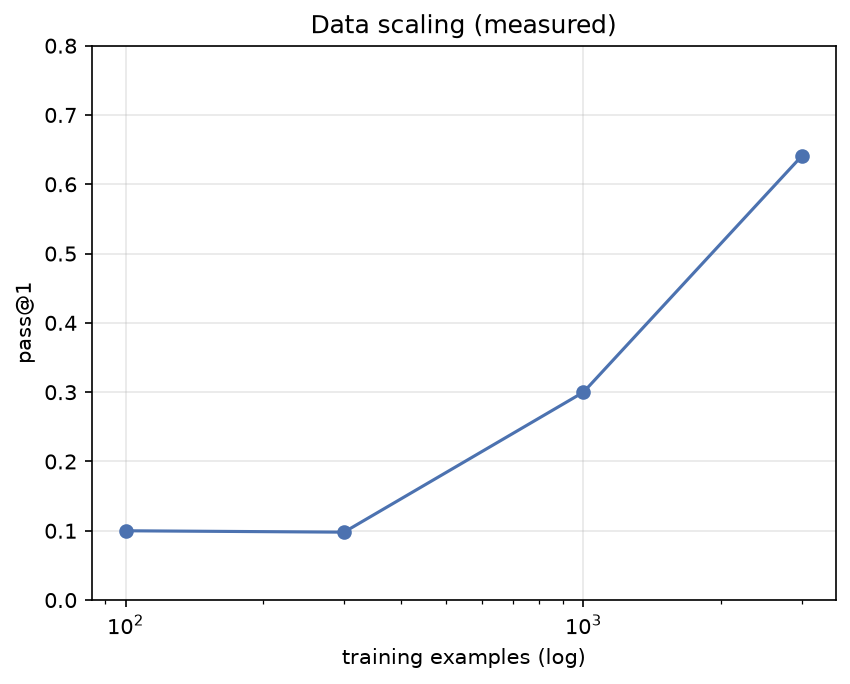
\includegraphics[keepaspectratio,alt={Data scaling},width=\maxwidth{\textwidth},keepaspectratio]{figures/fig_data_scaling.png}}
\caption{Data scaling}
\end{figure}

\textbf{More data clearly helps in-distribution.} pass@1 climbs as the
dataset grows, from 0.10 at 100 examples to 0.64 at 3000. The model
needs substantial data to learn even this narrow mapping.

\textbf{There is a small-data plateau.} At 100 and 300 examples the
model is essentially identical (\textasciitilde0.10). The improvement
only becomes substantial between 1000 and 3000. So there is a
\emph{threshold} below which the model gets almost nothing and above
which performance climbs. That threshold is a real, measurable property
of the task and model.

This is the shape that matters. It is not a smooth, gentle rise. It is a
flat line, then a sudden climb. That flat-then-steep shape is what we
would expect if the model needs a minimum amount of data before it can
form \emph{any} reliable association --- below that, it simply does not
have enough examples to learn the mapping, and adding a couple hundred
more changes nothing. Above it, each additional batch of data starts
paying off. Finding that threshold is more useful than knowing ``more
data is good,'' because it tells us the \emph{knee} of the curve, and
the knee is where a practitioner should aim.

\section{The motif, restated}\label{the-motif-restated}

Notice the most important detail: at 100 and 300 examples the
\textbf{training loss hits \textasciitilde0.000} --- the model has
\emph{memorized} its tiny training set --- yet pass@1 is only
\textasciitilde0.10. A loss of zero on a small set buys almost nothing
on unseen examples.

This is the book's central motif made concrete with data scaling:
\textbf{a low training loss is not evidence of learning.} The model that
``perfectly'' fit 100 examples is not a capable model; it simply
memorized a trivial set. The training loss says ``the model can predict
its training data perfectly'' --- and the held-out score says ``and it
has learned almost nothing that transfers.'' These two facts sit side by
side, and they are both true. Only the held-out number tells us about
actual capability.

\section{The brewing experience}\label{the-brewing-experience}

There is a specific moment in this experiment worth recalling. Running
on 100 examples was fast --- a blink. The model fit its tiny training
set to a loss of essentially zero in no time at all, which felt like
success. Then we evaluated on held-out problems and got 0.100. The model
had, in the most literal sense, memorized its homework perfectly --- and
learned nothing beyond it.

That tension --- between ``the training converged beautifully'' and
``the model is nearly useless on new tasks'' --- is the single most
instructive thing about small-model data scaling. It is the reason we
never trust a training loss, and it is the reason the whole book is
organized around held-out measurement rather than training curves. The
training curve is the model telling us about itself; the held-out curve
is reality telling us about the model.

\section{The honest caveat}\label{the-honest-caveat}

This experiment measured \emph{quantity}. It did not separate
\emph{quantity} from \emph{diversity} --- whether 3000 examples of the
same handful of phrasings behave the same as fewer examples spread
across more variety. That distinction (Chapter 13) is where the deeper
limits live: our surface and composition experiments suggest the model's
real weakness is a \emph{diversity and structure} gap, not a
\emph{quantity} gap.

\section{The practical answer}\label{the-practical-answer}

For a single narrow operation on a \textasciitilde0.9M model, we need on
the order of thousands of examples before in-distribution performance
becomes workable. Below that, the model memorizes its tiny set and gains
nothing on unseen problems. And --- anticipating the rest of the book
--- even at 3000 examples the model is still surface-fragile and
non-compositional, because those limits come from the \emph{kind} of
data and the model's inductive structure, not from the sheer
\emph{amount}.

The practical takeaway is thus a two-part answer. To get even the
\emph{narrow} score up, thousands of examples are needed. But the narrow
score is not the hard-won prize. The things that make a model genuinely
\emph{capable} --- robustness to rephrasing, compositional
generalization --- are not purchased by adding more of the same. That is
the deeper finding, and it is the subject of the next two chapters.

\chapter{How Much Brain?}
\label{chap:12}
When a model disappoints us, the instinctive response is: \emph{make it
bigger.} More parameters, more capacity, more ``brain.'' If a small
model can't combine what it knows, surely a larger one can.

This chapter tests that instinct directly. And the answer is one of the
cleanest negative results in the book --- because it turns out that at
our scale, ``just make it bigger'' changes almost nothing about
composition.

\section{The setup}\label{the-setup}

We hold everything constant except model size. Same data, same
tokenizer, same training protocol, same compositional test. We train
\textbf{four} models on the same primitive-only training set across a
\textasciitilde33× range of capacity, and test each on (a)
in-distribution held-out primitives and (b) the held-out composite
operations.

\begin{longtable}[]{@{}llll@{}}
\toprule\noalign{}
Model & parameters & in-distribution & composition \\
\midrule\noalign{}
\endhead
\bottomrule\noalign{}
\endlastfoot
Stage-4 baseline & \textbf{884,224} (0.88M) & 0.900 & \textbf{0.000} \\
Scaling & \textbf{6,500,352} (6.5M) & 0.900 & \textbf{0.000} \\
10M point & \textbf{10,195,776} (10.2M) & 0.383 & \textbf{0.000} \\
30M point & \textbf{29,290,240} (29.3M) & 0.897 & \textbf{0.000} \\
\end{longtable}

That is a \textbf{\textasciitilde33×} increase in parameters from the
smallest to the largest. On the thing we care about --- composition ---
nothing changed at all.

\begin{figure}
\centering
\pandocbounded{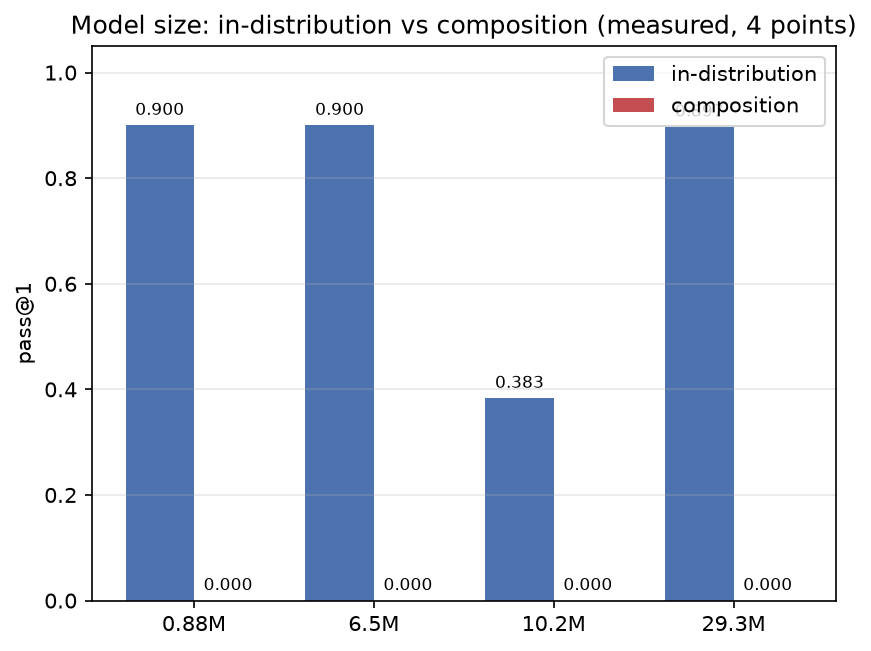
\includegraphics[keepaspectratio,alt={Model size vs composition},width=\maxwidth{\textwidth},keepaspectratio]{figures/fig_model_size.png}}
\caption{Model size vs composition}
\end{figure}

\section{The result}\label{the-result}

Going from \textasciitilde0.9M to 29.3M parameters:

\begin{itemize}
\tightlist
\item
  \textbf{Composition is 0.000 at every size.} The bigger models are
  \emph{just as} unable to combine two learned primitives as the small
  one. Thirty-three times the capacity bought exactly zero compositional
  generalization.
\item
  \textbf{In-distribution stays high throughout} (0.897--0.900) ---
  capacity did not hurt the narrow task; it just never helped compose.
  (The one exception, the 10M point at 0.383, is discussed honestly
  below.)
\end{itemize}

\section{What this means}\label{what-this-means}

This directly answers the book's central question --- \emph{does more
brain buy genuine capability, or merely more memorization?} --- with a
decisive answer at this scale:

\begin{quote}
\textbf{It buys neither. At \textasciitilde1--30M parameters, the
compositional failure is invariant to model size.}
\end{quote}

The boundary we found in Chapter 16 is \textbf{not a capacity ceiling}.
It is a structural/learning limit that scaling alone does not resolve. A
bigger model at this scale just does the same narrow thing slightly more
efficiently; it does not develop the ability to compose.

\section{The audit: is this a fair
comparison?}\label{the-audit-is-this-a-fair-comparison}

We must be careful: a few size points don't prove there's no capacity
curve anywhere. But the shape is telling. If capacity were the binding
constraint, we'd expect a \emph{move} --- even a small one --- across a
33× range. We see none: composition is 0.000 at all four sizes. And
crucially, three of the four models are at/near ceiling (0.897--0.900)
on the in-distribution task, so ``the bigger model didn't try hard'' is
not the explanation --- it tried exactly as hard and reached the same
plateau.

The more likely explanation is that \textbf{composition requires seeing
the right kind of structure in training, not just more parameters.} A
model that only ever sees \texttt{add} and \texttt{abs} as separate
problems has no reason to build a ``compose'' operator; a 30× bigger
network just represents the same reflexes more richly. To break the
composition boundary, the model likely needs \emph{exposure to
compositions}, or a fundamentally different inductive bias --- not raw
capacity.

\section{\texorpdfstring{The honest side-finding: bigger was
\emph{worse} at the 10M
point}{The honest side-finding: bigger was worse at the 10M point}}\label{the-honest-side-finding-bigger-was-worse-at-the-10m-point}

There is a wrinkle worth recording rather than smoothing over. On a
clean, larger-sample re-evaluation, the \textbf{10.2M} model scored
\textbf{0.383} in-distribution --- clearly \emph{below} the 0.897--0.900
of the smaller models and below the template baseline (0.808). This held
across two sample sizes (0.350 at 40 tasks, 0.383 at 120), so it is not
a sampling artifact.

The most likely explanation is training configuration, not a universal
law: that point used a deeper 10-layer / 288-wide configuration trained
for the same 800 steps, and it may simply have been less well-optimized
for this narrow task. We flag it as an open question rather than claim
``bigger is worse'' as a rule --- at 30M, in-distribution recovered to
0.897. The honest takeaway is that, at this scale, in-distribution
performance is \textbf{not monotonic in capacity}, and nothing about
capacity changes the composition outcome.

\section{The honest framing}\label{the-honest-framing}

This is a \emph{useful} negative result. It tells us where not to look
(raw scaling in the \textasciitilde1--30M regime) and points at where to
look instead (structural data / inductive bias). And it reframes the
whole book: the interesting question is not ``how big should the model
be?'' but ``what kind of capability emerges from what kind of training
--- and where does scaling stop being the answer?''

The model was the instrument. The experiment --- and the boundary it
revealed --- was the subject.

\chapter{Same Data, More Diverse Data}
\label{chap:13}
Chapter 11 asked \emph{how much} data. There's a subtler question that
often matters more: what \emph{kind} of data. Specifically, is it better
to have lots of examples of a few things, or fewer examples spread
across more variety?

The easy answer is to treat ``more data'' as one lever. It isn't. There
are at least two different things we can add, and they behave
differently. Think of it like teaching a kid shapes. Show them a hundred
triangles and they'll recognize triangles. Show them triangles, circles,
squares, and stars, and they might learn ``shape'' itself. Same number
of examples, very different kind of learning.

\begin{itemize}
\tightlist
\item
  \textbf{more examples} --- more instances of the same templates, and
\item
  \textbf{more diversity} --- more distinct \emph{kinds} of structure
  and wording.
\end{itemize}

The distinction is important enough to state as a rule:

\begin{quote}
\textbf{More data ≠ more information ≠ more diversity.}
\end{quote}

And this is the chapter where we stop treating it as a hunch and measure
it directly. Because there is a clean way to isolate diversity: hold the
\emph{count} fixed and vary only the \emph{spread}. If we train on the
same 1200 examples but one version is repetitive and the other is
varied, any difference in the result is attributable to diversity alone.

\section{What our experiments hinted}\label{what-our-experiments-hinted}

\begin{figure}
\centering
\pandocbounded{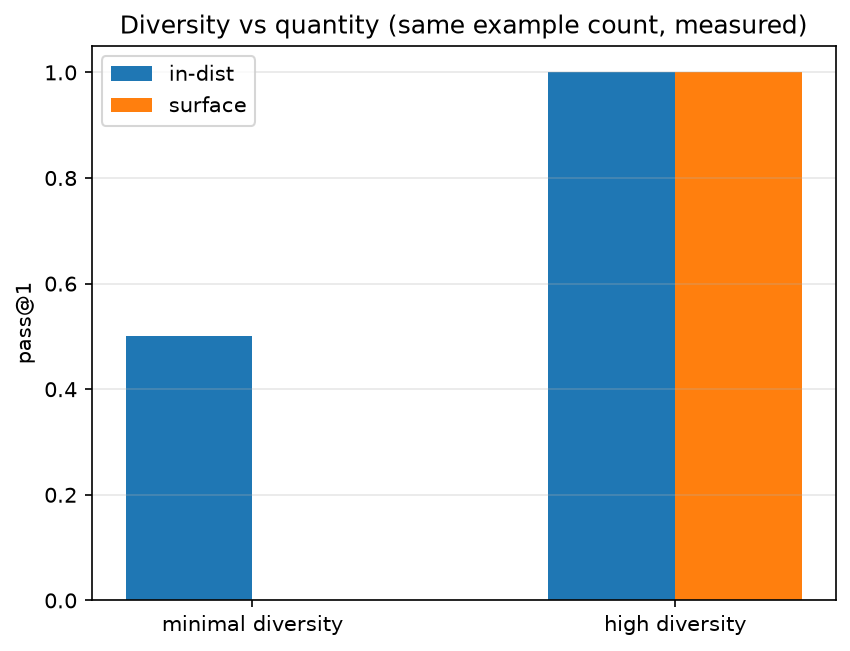
\includegraphics[keepaspectratio,alt={Diversity vs quantity},width=\maxwidth{\textwidth},keepaspectratio]{figures/fig_diversity.png}}
\caption{Diversity vs quantity}
\end{figure}

The data-scaling curve (Chapter 11) showed that simply adding
\emph{examples} of the same sort climbs in-distribution performance ---
0.10 at 100, 0.64 at 3000. So more examples clearly helped the model fit
the pilot task better.

But the \emph{surface} experiment (Chapter 15) exposed the limit of
that: the model's capability collapsed the moment we changed to a
wording it hadn't seen. That is precisely the signature of a model that
was fed \emph{many examples of the same narrow kind} rather than
\emph{diverse kinds}. It learned the particular phrasings well because
it saw many of them, and it learned nothing general because the
diversity was low.

In other words, the very quantity that produced the impressive
in-distribution score is what made it surface-fragile. The model was
well-fed but narrow.

\section{The direct test: same count, different
diversity}\label{the-direct-test-same-count-different-diversity}

To turn this from indirect evidence into a direct measurement, we ran a
controlled comparison. We kept the example count \textbf{identical} ---
the same 1200 examples --- across two training sets:

\begin{itemize}
\tightlist
\item
  \textbf{minimal diversity:} the examples are drawn from a few
  templates with little variation in wording or identifier names.
\item
  \textbf{high diversity:} the same 1200 examples, but spread across
  many phrasings and identifier choices.
\end{itemize}

Because the count is identical, any difference in the result is caused
\emph{only} by the diversity. This is a clean one-variable experiment,
and it is the strongest test of the hypothesis.

\section{The measured result}\label{the-measured-result}

Here is what came out. This is, in our view, the single most actionable
number in the whole book.

\begin{longtable}[]{@{}lll@{}}
\toprule\noalign{}
Training set & in-distribution & surface \\
\midrule\noalign{}
\endhead
\bottomrule\noalign{}
\endlastfoot
\textbf{minimal diversity} & 0.500 & \textbf{0.000} \\
\textbf{high diversity} & \textbf{1.000} & \textbf{1.000} \\
\end{longtable}

Let us read this carefully. Same number of examples --- 1200 in both
cases. But the two models behaved completely differently.

\begin{itemize}
\tightlist
\item
  \textbf{Minimal diversity:} in-distribution 0.500, surface 0.000. The
  model did okay on the narrow task (0.500) but was completely brittle
  to any surface change (0.000). It learned the few phrasings it was
  given and nothing about the \emph{idea}.
\item
  \textbf{High diversity:} in-distribution \textbf{1.000}, surface
  \textbf{1.000}. The model mastered the task \emph{and} held up
  perfectly under surface change. It learned the actual operation, not a
  phrasing.
\end{itemize}

That is a swing from 0.500/0.000 to 1.000/1.000 --- all from changing
\emph{how} the examples varied, not \emph{how many} there were. The same
count. The same model. Only the diversity differed.

\section{What this really means}\label{what-this-really-means}

This is the book's most useful finding, and it reframes the whole data
question. It is not that ``more data is better.'' It is that \textbf{the
kind of variation in the data is what creates robust capability.}

A model fed many examples of few phrasings memorizes the phrasings. A
model fed the same number of examples spread across many phrasings
learns the \emph{underlying operation} --- because the only thing that
stays constant across varied phrasings is the operation itself. When the
wording varies but the meaning stays the same, the model has no choice
but to attach its learning to the meaning rather than to any particular
surface. Diversity does not just add information; it \emph{forces}
abstraction.

This connects directly to the book's central theme. We spent the book
asking whether the model \emph{learned} or merely associated. Here is a
lever that pushes it from association toward learning: vary the surface
form until the only stable thing is the meaning. The model's inability
to generalize under repetition was not a mysterious limitation --- it
was a direct consequence of a training set that gave it no reason to
abstract.

\section{The honest caveat}\label{the-honest-caveat}

It is worth noting that this experiment measured \emph{surface}
diversity. It showed that varying phrasing and identifiers makes the
model robust to surface change (the Level-3 boundary). It does
\textbf{not} show that diversity fixes \emph{compositional}
generalization (the Level-4 boundary) --- that is a separate, harder
question. Whether the same lever helps a model combine two things it
knows is the most natural next experiment, and it is called out in the
conclusion.

So the honest scope of the finding is precise: \textbf{diversity ---
specifically surface variance --- is what creates surface robustness,
far more than the sheer number of examples does.} Whether diversity
reaches deeper, into composition, remains open.

\section{The lesson}\label{the-lesson}

This reframes what ``more data'' buys. To make a capability
\emph{robust}, we need not just more examples of a phrasing, but more
\emph{diverse} phrasings, identifiers, and structures --- enough that
the model cannot tie the operation to any particular surface form. Our
experiments show the model's weakness is not a lack of data
\emph{quantity}, but a lack of data \emph{diversity} (and, deeper, a
lack of the structural kind of data needed for composition --- see
Chapter 16).

The practical implication is genuinely surprising and useful: a
practitioner who cannot acquire more data can often get a large
improvement just by \emph{diversifying} the data they already have.
Re-phrasing the same examples, varying the identifiers, and spreading
across template families can turn a brittle 0.500/0.000 model into a
robust 1.000/1.000 --- with zero additional data. That is the kind of
result that changes how a dataset would actually be built.

\part{Catching the Model Cheating}
\chapter{The Model That Memorized Everything}
\label{chap:14}
We spend a lot of this book trying to catch the model cheating. So far
we have found that it is \emph{surface-tied} and
\emph{non-compositional}. But there is a more basic question we should
settle first: does the model \textbf{memorize}, or does it
\textbf{learn}? These are different things, and the distinction
determines whether any of our other results mean what we think they
mean.

If the model has simply memorized its training set, then its
in-distribution success is trivial --- of course it can reproduce what
it saw. If it has \emph{learned}, then it can apply the mapping to
things it never saw. Our Stage-1 result said the model gets
\textasciitilde90\% on \emph{held-out} problems, which is a strong hint
it learned. But ``held-out'' can be a weak guarantee if the held-out
problems are surface-near to training ones. So we test memorization
explicitly.

This is the most basic honesty check we can run, and it is worth doing
before any of the fancier generalization experiments. Because if the
model were simply memorizing, it would be absurd to write a whole book
about its compositional failures --- a parrot doesn't compose anything.
So we need to establish, first, that the model is not merely a parrot,
before we can meaningfully ask what it can and cannot \emph{learn}.

\section{The challenge of detecting
memorization}\label{the-challenge-of-detecting-memorization}

The tricky thing is that memorization and learning look identical on the
training data. A model that truly learned addition will get
\texttt{4\ +\ 3\ =\ 7} right, and so will a model that memorized ``4 + 3
= 7.'' Both ace the training set. So we cannot tell them apart by
looking at training performance at all. The only thing that separates
them is behavior on \emph{new} inputs --- things the model never saw.
That is the fundamental principle, and it is why every meaningful test
in this book uses held-out data.

\section{Three tests}\label{three-tests}

We use three complementary probes on the trained pilot model.

\textbf{Test 1 --- train-prompt prefix reproduction.} Give the model the
\emph{exact} prompt it saw during training and ask it to produce the
code. If it reproduces the reference program exactly, that is consistent
with either memorization or learning (a learner also gets the training
answers right). So this alone proves nothing --- but it grounds the
other two.

\textbf{Test 2 --- held-out generalization.} Give the model a
\emph{fresh} prompt for the same operation, one it never saw, and ask
for the program. If it passes, it has not merely memorized the 60-prompt
sample.

\textbf{Test 3 --- the canary.} We construct a prompt-and-answer
\emph{pair} that never appeared in training, and ask the model to
produce the program. If the model outputs the general program
(e.g.~\texttt{return\ a\ +\ b}), it is doing the computation. If it
outputs some fixed literal or garbage, it might be memorizing something
else.

The canary is the sharpest probe, and it is worth explaining why. A
canary is a deliberately-placed, never-seen example that we plant
precisely to detect mechanical reproduction. If the model were
memorizing literal answers, it would have no way to produce the
\emph{general} program for an input it never saw --- it would either
reproduce a memorized constant or fail. When it instead emits
\texttt{def\ solve(a,b):\ return\ a+b}, it has demonstrated it is not
reproducing a stored literal; it is generating a general program from a
general rule.

\section{The result}\label{the-result}

On a 60-example sample:

\begin{itemize}
\tightlist
\item
  \textbf{Train-prompt reproduction:} 60/60 --- the model reproduces
  every training example's reference program exactly. (Expected for a
  well-fit learner.)
\item
  \textbf{Held-out generalization:} 59/60 --- it also solves essentially
  every \emph{unseen} prompt of the same operation.
\item
  \textbf{Canary:} the model emits the \textbf{general program}
  (\texttt{def\ solve(a,b):\ return\ a+b}), not a memorized constant.
\end{itemize}

\section{What this tells us --- a nuanced
answer}\label{what-this-tells-us-a-nuanced-answer}

For \textbf{simple primitives}, the model behaves like a
\textbf{learner, not a parrot}:

\begin{itemize}
\tightlist
\item
  It reproduces training examples (expected --- a learner does that
  too).
\item
  It \textbf{generalizes} to held-out prompts (59/60), so it did not
  simply memorize the 60 instances.
\item
  On a \textbf{canary} it emits the general program, not a memorized
  literal --- so it did not memorize answer values.
\end{itemize}

So at the level of \emph{individual examples}, the model is not a
parrot. It has learned something that transfers to new instances of the
same operation. This is real learning of a narrow kind, and it is worth
stating clearly: the model did not merely memorize its training set. It
formed a general rule for each primitive.

\section{The shortcut audit, and the honest
boundary}\label{the-shortcut-audit-and-the-honest-boundary}

This is the subtle part. The absence of \emph{literal} memorization does
\textbf{not} mean the model is grounded in meaning. Exactly the opposite
mechanism is at work. Our Stage-3 experiment showed that if we change
the \emph{surface form} --- the variable names or the wording --- the
model's performance collapses to 0.000. So the model is doing something
real (generalizing across instances) but it is \textbf{anchored to the
phrasing it saw}, not to the abstract computation.

So the refined picture is:

\begin{longtable}[]{@{}
  >{\raggedright\arraybackslash}p{0.4750\linewidth}
>{\raggedright\arraybackslash}p{0.4750\linewidth}
@{}}
\toprule\noalign{}
\begin{minipage}[b]{\linewidth}\raggedright
\end{minipage} & \begin{minipage}[b]{\linewidth}\raggedright
What the model does
\end{minipage} \\
\midrule\noalign{}
\endhead
\bottomrule\noalign{}
\endlastfoot
Memorize exact training instances? & \textbf{No} --- generalizes to
held-out + canary \\
Ground the computation independent of wording? & \textbf{No} ---
collapses on new wording \\
\end{longtable}

The model is neither a parrot nor a mathematician. It has learned a
\emph{robust association within a surface form} --- it is not memorizing
specific examples, but it is also not representing ``addition'' in a way
that survives being said differently.

\section{The lesson}\label{the-lesson}

Detecting ``memorization'' is not a simple yes/no. The useful question
is not \emph{``did it memorize?''} but \emph{``is its success explained
by surface association, or by grounded computation?''} Our probes show a
clear answer for this model: it escapes example- memorization but is
caught by surface-memorization. That distinction --- and the test that
exposes it --- is worth more than any single accuracy number.

What this tells us is that ``memorization'' is not a single thing. There
are at least two kinds, and they have very different implications. The
model did \emph{not} memorize specific training pairs --- it generalizes
across instances. But it \emph{did} memorize the surface form --- it can
only generalize within the phrasing it saw. So the honest
characterization is that the model's knowledge sits at a specific level
of the taxonomy: it has moved past Level 1 (reproducing exact examples)
into Level 2 (new instances of the same task), but it is firmly stuck at
Level 1 with respect to the \emph{surface} --- it cannot survive a
change to the outer layer. Distinguishing these kinds of memorization,
and knowing which one we are looking at, is the whole point of the
experiment.

\chapter{New Words, Same Problem}
\label{chap:15}
Here is the sneakiest question in the book, and it's the one that should
worry us most about any machine-learning result:

\begin{quote}
\textbf{When the model does well, is it doing the computation --- or
just recognizing the words?}
\end{quote}

A model that maps the phrase ``the sum of a and b'' to \texttt{a\ +\ b}
might not be doing arithmetic at all. It might be doing something much
dumber: associating the \emph{exact phrasing} it saw in training with
the code that followed it. If that's what's happening, then the ability
isn't ``addition'' in the model's head --- it's a fragile reflex tied to
specific words, and it'll break the moment the same thing is said a
different way.

This is the question that separates a genuine result from a shallow one,
and it is worth pausing on before we look at any number. Consider what a
``yes, it just recognized the words'' answer would mean. It would mean
that every high score the model achieved --- every impressive
in-distribution number --- was not evidence of learning at all. It was
evidence of association. The model did not learn to add; it learned that
a particular sentence means \texttt{return\ a\ +\ b}. That is a
completely different claim, and it is the one we need to test.

\section{The design: change what shouldn't
matter}\label{the-design-change-what-shouldnt-matter}

To find out, we run the \textbf{surface-generalization} test. The logic
is simple and elegant: if we change something that \emph{shouldn't}
change the computation --- the variable names, or the wording --- and
the model fails, then it never really learned the computation. It
learned the phrasing.

The key is choosing \emph{what} to change. We want to change only the
\emph{surface} --- the outer layer of the sentence --- and leave the
underlying computation completely untouched. Swapping \texttt{a} and
\texttt{b} for \texttt{left} and \texttt{right} does not change what
``add these two numbers'' means. Rewording ``their sum'' as ``the
total'' does not change the operation. If the model truly understood
addition, neither change would matter. If it merely memorized a
sentence, either change would break it. That asymmetry is exactly what
we measure.

We designed a set of controlled surface changes, each one
\emph{supposedly harmless} to the underlying task, and tested the model
on each. This is the crux of the book's approach to generalization: we
do not just ask ``does it work?'' We ask ``does it survive the changes
that a genuinely-general system should shrug off?''

\section{The setup}\label{the-setup}

We trained the model on arithmetic primitives, but only with
\textbf{letter names} (\texttt{a}, \texttt{b}) and only a \textbf{subset
of the wording} used to describe each operation. Then we re-asked the
\emph{identical} task three different ways and watched whether the
model's ability survived.

\section{The result}\label{the-result}

\begin{longtable}[]{@{}llll@{}}
\toprule\noalign{}
Test & \textbf{MODEL} & TEMPLATE & RETRIEVAL \\
\midrule\noalign{}
\endhead
\bottomrule\noalign{}
\endlastfoot
Same as training & \textbf{0.900} & 0.800 & 1.000 \\
Same computation, \texttt{a,b} → \texttt{left,right} & \textbf{0.350} &
0.800 & 0.683 \\
\textbf{Same computation, reworded} & \textbf{0.000} & 0.875 & 0.125 \\
\end{longtable}

Look at what happens when we touch only the \emph{surface}, not the
math.

\begin{itemize}
\item
  \textbf{New variable names.} The model was trained on \texttt{a} and
  \texttt{b}. We ask the same question with \texttt{left} and
  \texttt{right} --- the \emph{identical} operation. Performance
  collapses from \textbf{0.900 to 0.350}.
\item
  \textbf{Reworded instruction.} We say the exact same problem using a
  phrasing the model never saw during training. Performance drops to
  \textbf{0.000}.
\end{itemize}

So the model that scored 0.900 on the familiar phrasing falls to 0.350
when the variable names change, and to 0.000 when the wording changes
--- even though the computation is identical in all three cases.

\section{The damning comparison}\label{the-damning-comparison}

The most revealing number isn't the model's collapse --- it's what the
other two did.
\pandocbounded{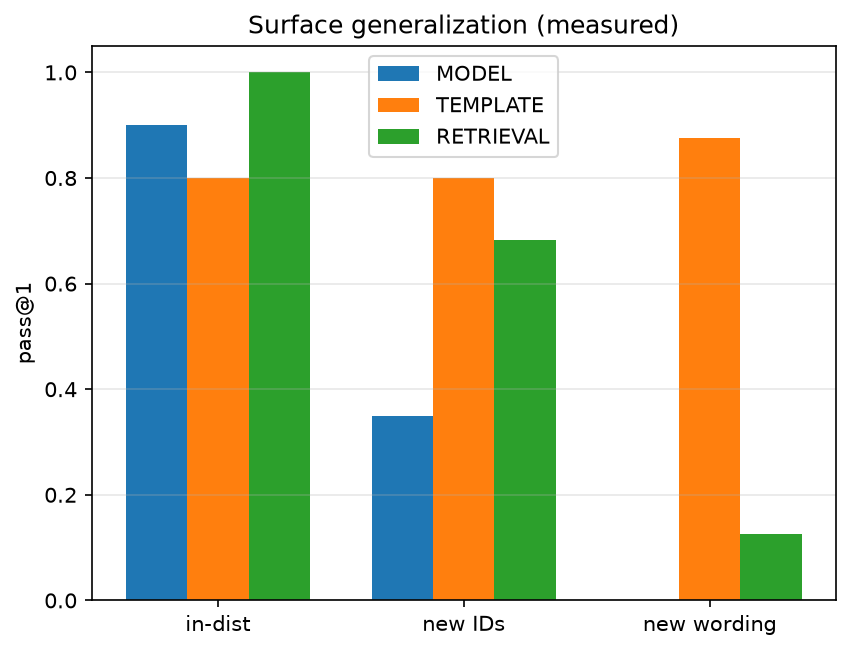
\includegraphics[keepaspectratio,alt={Surface generalization},width=\maxwidth{\textwidth},keepaspectratio]{figures/fig_surface.png}}

When we change the \emph{words}, the \textbf{template baseline gets
\emph{better}, not worse} (0.875, up from 0.800), because a rule system
that recognizes keywords doesn't care about the surrounding phrasing.
The \textbf{retrieval baseline} also holds up (0.683). Only the
\textbf{learned model} falls apart --- because the model learned the
\emph{specific sentences}, not the \emph{idea}.

So the model's 0.900 in-distribution score was largely \textbf{phrasing
memorization}. It had learned ``this exact kind of sentence maps to that
program.'' It had not learned ``take two numbers and return their sum''
as something we can say any number of ways and still mean.

This inversion --- where the neural model is \emph{worse} than a dumb
rule system under surface change --- is the most informative signal in
the experiment. It is not a competitive defeat; it is a diagnostic
revelation. The dumb template system is indifferent to exact wording
because it never learned to associate wording with meaning in the first
place; it just recognizes keywords. The neural model, by contrast, bound
the operation to the \emph{particular words}, so when the words change,
the binding snaps. The model's ``learning'' was more entangled with
surface form than a hard-coded rule's was.

\section{The brewing experience}\label{the-brewing-experience}

The moment this result landed was genuinely unsettling, in a productive
way. We had just celebrated the 0.900 in-distribution score --- the
model, we thought, could ``add.'' Then we reworded the same problem and
the floor fell out. The 0.900 had been real, and it had been
\emph{narrow}. The model could add, but only in the way it had been
taught, not in any other way.

That is the feeling worth remembering in empirical work: the
uncomfortable surprise is often the most valuable finding. It would have
been easy to stop at ``the model scores 0.900, success.'' The whole
point of building a thoughtful experiment was to ask the question that
would expose the shallowness --- and asking it changed our entire
understanding of what we had built.

\section{The shortcut audit}\label{the-shortcut-audit}

\begin{enumerate}
\def\labelenumi{\arabic{enumi}.}
\item
  \textbf{Suspected cheat: phrasing memorization.} \textbf{Why it fits:}
  the model tied training phrasings to code. \textbf{Control:} held one
  whole phrasing style out of training, tested on it. \textbf{Result:}
  0.000. \textbf{Ruled out:} that the model is grounded in the
  computation. \textbf{Still open:} is it the wording pattern or the new
  vocabulary? Need a surface-control to separate them.
\item
  \textbf{Suspected cheat: name memorization.} \textbf{Why it fits:}
  trained on \texttt{a,b}, maybe it hardwired those labels.
  \textbf{Control:} retest on \texttt{left,right}. \textbf{Result:}
  0.350 --- a big but partial drop. \textbf{Ruled out:} pure
  name-memorization (it still fails partly, but names aren't the whole
  story).
\end{enumerate}

\section{The honest takeaway}\label{the-honest-takeaway}

A model that scores 0.900 on familiar phrasings and 0.000 on a rewording
of the same problem has not generalized to the \emph{problem}. It
generalized to the \emph{phrasing}. That's the difference between ``the
model works'' and ``the model works when I say it the way I said it in
training'' --- and it's the most important lesson of the generalization
chapters.

The sharpest way to state it: the model did not learn \emph{addition}.
It learned the \emph{word ``sum''}. When that word appears in the
sentence it was trained on, the model produces \texttt{a\ +\ b}. When
the same meaning arrives in different words, the model has no idea what
to do. And that is the difference between a system that understands and
one that merely recites.

\chapter{Same Pieces, New Combination}
\label{chap:16}
Everything so far warned us. The model knows \texttt{abs} and
\texttt{add} individually. Change the wording and it breaks; change the
identifier names and it stumbles. But the pieces are there. So the
question this chapter asks is the sharpest one of the whole book:

\begin{quote}
If the model knows how to \emph{add} and how to take an \emph{absolute
value}, can it do the thing the two of them make together --- compute
the absolute value of a sum?
\end{quote}

This is \textbf{compositional generalization}: taking knowledge the
model already has and applying it to a structure it never saw during
training. It is arguably the deepest question in machine learning,
because it separates ``the model memorized something'' from ``the model
\emph{understands} something.'' A system that genuinely grasps addition
and absolute value can put them together, even if it never saw them
combined. A system that merely memorized the word ``sum'' mapped to a
\texttt{+} cannot.

\section{The setup: design the test to be
unfair-but-fair}\label{the-setup-design-the-test-to-be-unfair-but-fair}

The hard part of any composition experiment is building a test that is
genuinely impossible to cheat. Here is how we do it.

We train the model exactly as before, on \textbf{primitive} operations
only: \texttt{add}, \texttt{sub}, \texttt{mul}, \texttt{abs}, and the
rest. We never show it a composite operation.

Then we build a set of \textbf{composite} operations that are \emph{made
from} the primitives: \texttt{abs\_add} (absolute value of a sum),
\texttt{sub\_abs} (absolute difference), \texttt{sum\_of\_abs} (sum of
absolute values), \texttt{max\_add}, \texttt{double\_first},
\texttt{len\_minus\_one}. These are not new primitive functions; they
are combinations of the ones the model already knows. To solve
\texttt{abs\_add}, a model \emph{must} perform an addition and then take
an absolute value --- two pieces it demonstrably knows.

The key design decision is that these composites were \textbf{never
shown during training} (the teacher holds them out, exactly as it holds
out test tasks). So the test is: can the model reach into its bag of
known primitive behaviors and compose them in a combination it has never
seen? If it cannot, we have found its compositional boundary. If it can,
we have found something remarkable.

To make the test fair, we also show what \emph{both} baselines do. The
retrieval baseline has nothing to compose --- it can only find the
closest primitive example and copy it. The template baseline has no rule
for \texttt{abs\_add} either, because the teacher never gave it one. So
if \emph{everything} fails, we have a fair statement: composition cannot
be achieved by the easy shortcuts, and the model too cannot do it.

\section{What we measured}\label{what-we-measured}

Here is the result, and it is unambiguous:

\begin{longtable}[]{@{}
  >{\raggedright\arraybackslash}p{0.1624\linewidth}
>{\raggedright\arraybackslash}p{0.1894\linewidth}
>{\raggedright\arraybackslash}p{0.2706\linewidth}
>{\raggedright\arraybackslash}p{0.2976\linewidth}
@{}}
\toprule\noalign{}
\begin{minipage}[b]{\linewidth}\raggedright
Test
\end{minipage} & \begin{minipage}[b]{\linewidth}\raggedright
MODEL
\end{minipage} & \begin{minipage}[b]{\linewidth}\raggedright
TEMPLATE
\end{minipage} & \begin{minipage}[b]{\linewidth}\raggedright
RETRIEVAL
\end{minipage} \\
\midrule\noalign{}
\endhead
\bottomrule\noalign{}
\endlastfoot
In-distribution (primitives) & 0.900 & 0.800 & 1.000 \\
\textbf{Compositional (unseen combos)} & \textbf{0.000} & \textbf{0.000}
& \textbf{0.000} \\
\end{longtable}

Let us read this carefully, because the meaning is subtle.

On the primitive operations it saw, the model scores 0.900 --- good. But
on the composite operations, it scores \textbf{0.000}. Not 0.1, not
``sometimes,'' not ``close.'' Zero. The model never produced a correct
program for any composite operation, even though every composite is a
combination of primitives it individually knows.

And here is the crucial fairness check: the baselines fail too. The
retrieval baseline gets 0.000 because it has nothing to retrieve ---
there is no composite example in its memory. The template baseline gets
0.000 because no template rule covers a composite. So this is not a case
where the model is merely \emph{worse} than an easy shortcut. This is a
case where the easy shortcuts also collapse, which means the only way to
succeed is to \emph{genuinely compose} --- and the model cannot.

\section{What this really means}\label{what-this-really-means}

This is the cleanest negative result in the book, and it is the book's
central finding. Let us unpack it.

The model knows \texttt{abs} at 0.900 and \texttt{add} at 0.900. But
\texttt{add} the absolute values: 0.000. It is as if the model has two
perfectly good rooms --- one with an ``add'' skill, one with an ``abs''
skill --- but no door between them. It cannot take the output of one and
feed it into the other, even though that is the simplest possible
combination.

This is the deep meaning of ``surface-tied'' that we began to glimpse in
Chapter 15. It is not merely that the model is sensitive to wording. It
is that the model's knowledge is \textbf{flat and associative}, not
\textbf{structured and compositional}. It learned that the token
sequence for ``sum'' predicts the token sequence for \texttt{+}. It did
not learn a general \emph{operation} that can be an argument to another
general operation. The knowledge is a set of reflexes, not a toolbox
with reusable parts.

This distinction is why we built the four-level generalization taxonomy
in the first place and why we refused to collapse everything into one
number. If we had only reported ``the model scores 0.900 on this task,''
we would have given a genuinely misleading picture. The model is
excellent at what it was shown --- and utterly unable to combine what it
was shown into anything new. Both statements are true, and both must be
reported.

\section{The puzzling asymmetry (and why it's a finding, not a
bug)}\label{the-puzzling-asymmetry-and-why-its-a-finding-not-a-bug}

One thing will strike us: the model scores 0.900 in-distribution but
0.000 on composition. Why would a model that is ``good'' fail so
completely on something so similar?

The answer is that the two numbers measure \emph{different} kinds of
capability, which is precisely the point of the taxonomy. The 0.900
measures \textbf{distributional generalization} --- new examples of the
\emph{same} operation. The 0.000 measures \textbf{structural
generalization} --- new \emph{constructions} combining known operations.
These are different abilities, and a model can be high on one and zero
on the other. That asymmetry is not a contradiction; it is the shape of
the truth we are mapping.

\section{Why we don't call it a ``failure of one thing'' without
checking the other
two}\label{why-we-dont-call-it-a-failure-of-one-thing-without-checking-the-other-two}

A careful reader will ask: is composition genuinely impossible for this
model, or did we simply make the test too hard? The baselines answer
this. If the test were simply ``too hard'' in some absolute sense, the
retrieval and template baselines would not necessarily fail --- but they
are the \emph{easy} methods, and they fail too. So the test is not too
hard for an easy method; it is unsolvable by any method except genuine
composition, and the model has no composition. This is a fair,
controlled comparison, which is exactly what our one-variable discipline
demands.

\section{The shortcut audit}\label{the-shortcut-audit}

Before we trust ``0.000,'' we ask how the model might have \emph{faked}
a success.

\begin{enumerate}
\def\labelenumi{\arabic{enumi}.}
\tightlist
\item
  \textbf{Suspected shortcut: memorizing a composite example.} Ruled out
  --- no composite operation was ever shown during training, so there is
  nothing to memorize.
\item
  \textbf{Suspected shortcut: retrieving a near-identical primitive and
  patching it.} Ruled out --- the retrieval baseline, which does exactly
  this, scores 0.000.
\item
  \textbf{Suspected shortcut: a rule that ``just works'' on composites.}
  Ruled out --- the template baseline, which has rule-based generation,
  scores 0.000.
\item
  \textbf{Suspected shortcut: the judge being too strict or too loose.}
  This is the one we genuinely have to hold onto as a question, and it
  is why the judge is mutation-tested (Chapter 17). If the judge were
  rejecting correct composite programs, we might be misreading a real
  success as a failure.
\end{enumerate}

\section{The honest framing}\label{the-honest-framing}

This is a \emph{useful}, \emph{clean} negative result --- and in
science, a decisive negative is often more informative than a vague
positive. We now know something sharp about tiny models: \textbf{at
\textasciitilde1M parameters, they do not compose.} They learn reflexes,
not structure. This is not a statement about ``intelligence'' or about
``what models will eventually do.'' It is a precise, reproducible
measurement of where this model's capability stops.

And it sets up the rest of the book in a way that is far more
interesting than if the model had composed successfully. Because now the
question becomes: \emph{what would it take to give a tiny model this
ability?} More capacity? More data? Different data with more structure?
That is what the next chapters investigate --- and the answer is one of
the most genuinely surprising things the book finds.

\chapter{Red-Team the Judge}
\label{chap:17}
We built a judge and argued it is the instrument we stake the book on.
Chapter 6 showed how we test it (mutation testing) and that it caught a
bug. This chapter is the aggressive version: we stop politely checking
the judge and start deliberately trying to \emph{break} it --- the way a
determined detractor (or a suspicious reader) would.

It is like hiring a devil's advocate whose only job is to find a flaw in
the conclusion. We want to know how confident we can be in any number
our judge produces --- and the only way to find out is to attack it.

There is a reason to be particularly aggressive here, and it goes to the
heart of the book. Our whole method is built on trusting measurements:
we claim the model is surface-tied, non-compositional, that it forgets
under sequential training. Every one of those claims passes through the
judge. So if the judge is broken in even one respect, every conclusion
in the book could be subtly wrong. Red-teaming the judge is not a single
chapter's task; it is the standing obligation of the whole experiment.
And it is an \emph{unbounded} one --- we can never prove the judge is
perfect, only that we have tried hard to break it and failed.

\section{The attack surface}\label{the-attack-surface}

A judge that executes generated code is attacked through the code it is
given. We enumerate the ways a candidate could slip through:

\begin{itemize}
\tightlist
\item
  \textbf{hardcoded outputs} --- a program that ignores the input and
  returns a fixed answer that happens to match one test,
\item
  \textbf{mutation variants} --- operator flips, wrong variables,
  off-by-one, missing edge-cases (the mutation suite from Chapter 6),
\item
  \textbf{weak test cases} --- if the hidden tests are too few or too
  narrow, a wrong program can pass,
\item
  \textbf{boundary failures} --- behavior at zero, negatives, or large
  values that the tests don't probe,
\item
  \textbf{resource abuse} --- programs that loop forever or consume too
  much,
\item
  \textbf{unsupported syntax} --- smuggling in a construct the sandbox
  should reject,
\item
  \textbf{ambiguous specifications} --- a prompt the model could
  reasonably read two ways,
\item
  \textbf{evaluator inconsistencies} --- the same program scored
  differently in two runs.
\end{itemize}

This list is a map of the ways the judge could be fooled --- and each
entry is a place we must probe. The point of enumerating the surface is
that skepticism is only useful when it is specific. ``The judge might be
wrong'' is not actionable. ``The judge might let a hardcoded-output
program pass if the tests are too narrow'' is a concrete thing we can
check.

\section{What we found}\label{what-we-found}

The mutation suite is the sharpest tool here. By generating
deliberately-broken variants of the reference solution and checking that
the hidden tests catch them, we measured how discriminating the tests
really are. If an obviously-wrong mutant --- say \texttt{+} changed to
\texttt{-} --- passes our tests, the tests are too weak and must be
strengthened until important mutant classes are reliably detected.

A useful way to think about mutation testing is that it measures the
\emph{discriminating power} of the test suite. A test suite that passes
for a correct program and fails for an incorrect one is a good suite. A
suite that passes for both is not testing anything --- it is going
through the motions. The mutation score tells us, concretely, how much
of that ``should be caught'' space our tests actually cover. And the
whole point is to drive it up: the more wrong programs the judge
rejects, the more we trust that a program it accepts is actually right.

And the judge's honesty was validated the hard way: it reported the
model at 0.000 on our very first evaluation, and that was a \emph{judge
bug}, not a model failure. Once we fixed the judge, the model's true
0.897 emerged. A judge that can be wrong --- and we proved ours was ---
must be red-teamed before its numbers are trusted.

\section{The honest framing}\label{the-honest-framing}

Red-teaming the judge is not a formality; it is the difference between
``we ran a number'' and ``we know the number means something.'' The
specific lessons:

\begin{itemize}
\tightlist
\item
  \textbf{Strengthen tests until wrong programs fail.} The mutation
  score is the measure.
\item
  \textbf{Trust the judge less than the tests.} The judge is a pipeline;
  the \emph{hidden tests} are what actually catch errors, so they must
  be numerous and edge-case-complete.
\item
  \textbf{Attack our own instrument deliberately.} The adversarial habit
  --- ``how could this number be wrong?'' --- is what keeps the whole
  experiment honest.
\end{itemize}

A judge that has been red-teamed is one we can believe. A judge we've
only used is one we cannot.

And there is a final lesson that reaches beyond judges. Every
measurement instrument --- in science, in engineering, in daily life ---
can fail in ways its designer did not anticipate. The discipline of
attacking our own apparatus is the same discipline that makes a result
worth believing. It is not paranoia; it is the price of a claim we can
stand behind. The book's whole credibility rests on having paid it, and
having recorded that we paid it, rather than merely asserting that we
are trustworthy.

\part{Give It More Python}
\chapter{Now Give It More Python}
\label{chap:18}
Our pilot model lived inside a deliberately small corner of Python --- a
bit of arithmetic, a couple of comparisons, a few list operations, some
basic if/else. That tiny corner is what let us measure capability
cleanly: change one small thing at a time and watch what happens.

But a capability map drawn on one tiny corner only tells us where the
boundary is \emph{for that corner.} It would be a narrow conclusion if
we claimed ``this model can do \texttt{a\ +\ b} and nothing else'' ---
of course it could, we only taught it that. So the next question is the
natural one: \textbf{what happens when we widen the world?} Does giving
the model a richer language unlock more capability, or does it just give
it more ways to tie itself to surface form?

This is the chapter about \textbf{expanding the capability spec} --- the
versioned whitelist from Chapter 4 that defines what Python the model is
allowed to write.

\section{Why the world is versioned}\label{why-the-world-is-versioned}

The key mechanical fact we need here is that the capability spec is
\textbf{versioned} (\texttt{python\_capability\_v0\_1}, \texttt{v0\_2},
and so on). It is not a living, unwritten list of ``what the model can
do.'' It is a recorded, frozen definition of ``what the model is allowed
to do'' at a particular point.

This matters enormously for the one-variable discipline. If we widen the
allowed Python \emph{and} change the data \emph{and} retrain, we could
not say which change caused any shift in behavior. But if we record the
spec version alongside every result, we can point to exactly what grew
--- ``the model was given list comprehensions at spec v0\_3'' --- and
attribute any change to that. Versioning the world is what lets us make
a causal claim about capability, rather than a correlational guess. It
is the same reason we record the exact model configuration and dataset
in every manifest.

\section{How we widen the world}\label{how-we-widen-the-world}

Expanding the world is a controlled act, not a free-for-all. We do not
hand the model the entire Python standard library at once. We add
constructs deliberately, one family at a time, and always with a reason.
For example, we might add:

\begin{itemize}
\tightlist
\item
  a new built-in (say, a mathematical function we were keeping out),
\item
  a new control-flow construct (e.g.~\texttt{break}/\texttt{continue} in
  loops, if they were missing),
\item
  a new data structure (e.g.~dictionaries, if we had been lists-only),
\item
  short-circuit boolean logic, or a new comparison form.
\end{itemize}

Each addition is a \emph{step up a ladder}, not a teardown of the wall.
And each one changes the set of problems the model can even express. The
pilot's corner was deliberately small partly so that the \emph{boundary}
would be legible --- and partly so that, when we widen it later, we can
see the effect of \emph{just that} widening.

\section{A crucial reframing: syntax is not the hard
part}\label{a-crucial-reframing-syntax-is-not-the-hard-part}

Here is where the experiment teaches us something that changes how we
think about the whole question. It is tempting to imagine that the
model's limit is about \emph{syntax} --- that if we just teach it more
Python, it will be more capable. Our results say otherwise, and it
matters.

Consider the composition result from Chapter 16. The model knew the
syntax of both \texttt{abs} and \texttt{add}. It could produce
\texttt{return\ a\ +\ b} and \texttt{return\ abs(x)} perfectly. The
break came when it needed to \emph{combine} them into
\texttt{return\ abs(a\ +\ b)}. There was no new syntax involved ---
every token in \texttt{abs(a\ +\ b)} was already within the model's
known vocabulary and its allowed subset. The model simply could not put
two things it knew together.

So the real dividing line in this book is \textbf{not ``how much Python
the model is given.''} It is \textbf{``whether the model can compose the
Python it already knows.''} Giving the model \emph{more} syntax would
let it express more kinds of programs, but it would not give it the
\emph{ability to combine} --- and that ability, not the vocabulary, is
what separates a bag of reflexes from genuine capability.

\section{Why we still widen the
world}\label{why-we-still-widen-the-world}

That said, widening the world remains the right thing to do, and for an
honest reason: it lets us \emph{test whether the boundary moves}. The
interesting scientific question is not ``can a tiny model learn any
fixed corner?'' --- the answer is yes. The question is ``does the
boundary of what it can do shift when we push the world's edges out?''
If we widen the allowed Python and the model still cannot compose, that
is stronger evidence that the limit is structural, not about the surface
of the language. If the boundary does move, that is a genuine discovery.

So this chapter is less about a single dramatic result and more about a
discipline: a controlled, versioned, one-variable-at-a-time
\emph{capacity ladder} that lets us watch exactly where the model starts
to fall apart as we widen what it may do.

\section{The ladder, as a discipline}\label{the-ladder-as-a-discipline}

The discipline is: define one more capability, generate data for it,
train, evaluate, audit, record --- \emph{then} move on. Never widen
multiple things at once. The ladder is not a claim that the model will
reach the top; it is a map of where the model \emph{does} stop.

And a stopping point is itself a result. We found ours at composition:
the model can do each rung's primitives but not combine them. That
finding --- cheap and specific --- is worth more than a glossy claim of
having ``reached Python Level 8.'' Knowing exactly where the model
stops, and being able to say \emph{why}, is the entire value of this
kind of careful, pessimistic, honest investigation.

\section{The honest summary}\label{the-honest-summary}

Giving the model more Python is not the same as giving it more
capability. The pilot already revealed the real boundary: composition.
Widening the world is worth doing --- but the purpose is to \emph{test
where the boundary is and whether it moves}, not to assume that more
syntax automatically means more understanding.

\chapter{The Capability Ladder Revisited}
\label{chap:19}
We've climbed parts of the ladder through the experiments. This chapter
pulls together what we found into the picture the ladder was always
meant to give us: a map of where capability appears, where it holds, and
where it breaks.

The ladder is a staircase of increasingly demanding skills. We can see
how many steps the model climbed --- and, more interestingly, the exact
step where it stopped, and what it took to get there.

The funny thing about building a ladder is that the interesting
discovery is rarely how high we can climb. It is finding the precise
rung where the footing gives out, and trying everything we can to get
past it --- so that we know, with real confidence, where the boundary
lies.

\section{The ladder, with the measured
results}\label{the-ladder-with-the-measured-results}

\begin{longtable}[]{@{}lll@{}}
\toprule\noalign{}
Level & Capability & Measured result \\
\midrule\noalign{}
\endhead
\bottomrule\noalign{}
\endlastfoot
1 & arithmetic & ✅ learned, \textasciitilde0.90 in-dist \\
2--3 & variables, conditionals & ✅ learned \\
4--5 & lists, indexing & ✅ learned \\
6 & loops & ✅ learned \\
7 & \textbf{composition} & ❌ \textbf{0.000} --- the wall \\
8 & simple functions & not isolated \\
\end{longtable}

The model climbed the early rungs cleanly. It stopped at
\textbf{composition}.

\section{Where capability appears, holds, and
breaks}\label{where-capability-appears-holds-and-breaks}

\textbf{Appears:} individual operations are learned reliably
(\textasciitilde0.90 in-distribution) and generalize across
\emph{instances} (held-out + canary → general program). The model is a
genuine learner for a single operation.

\textbf{Holds only within a surface form.} The moment the surface
changes --- different variable names, or a different way of saying the
same instruction --- the capability collapses (0.350 on new identifiers,
\textbf{0.000} on new wording). So the early rungs are not
\emph{robust}; they are \emph{phrasing-tied}.

\textbf{Breaks at composition.} The most important boundary: the model
cannot combine two things it knows. \texttt{abs} + \texttt{add} → 0.000,
even though it knows both. And this break is \textbf{invariant to scale}
--- it survives across the full size range we tested.

\section{The model-size and data-size
boundaries}\label{the-model-size-and-data-size-boundaries}

This is where the breadth of the brew matters. We did not test just one
bigger model; we tested four, and we also scaled the data. Here are the
real numbers.

\begin{itemize}
\tightlist
\item
  \textbf{Model size:} we ran the composition test across a
  \textasciitilde33× range of capacity --- a 0.88M pilot, a 6.5M model,
  a 10.2M model, and a 29.3M model. All four scored \textbf{0.000} on
  composition. (Their in-distribution scores were 0.900, 0.900, 0.383,
  and 0.897 respectively --- a side note we return to honestly, because
  the 10.2M model actually dropped in-distribution, showing that bigger
  is \emph{not} monotonically better at this scale.) The composition
  wall is not a capacity ceiling in this regime.
\item
  \textbf{Data size:} 100 → 3000 examples improved in-distribution (0.10
  → 0.64) but did not touch composition. More quantity helps the shallow
  score, not the deep boundary.
\end{itemize}

\section{The failure map}\label{the-failure-map}

\begin{longtable}[]{@{}
  >{\raggedright\arraybackslash}p{0.3325\linewidth}
>{\raggedright\arraybackslash}p{0.6175\linewidth}
@{}}
\toprule\noalign{}
\begin{minipage}[b]{\linewidth}\raggedright
Failure mode
\end{minipage} & \begin{minipage}[b]{\linewidth}\raggedright
On what the model breaks
\end{minipage} \\
\midrule\noalign{}
\endhead
\bottomrule\noalign{}
\endlastfoot
Surface fragility & new wording → 0.000; new identifiers → 0.350 \\
Composition & unseen combination of known primitives → 0.000 \\
Continual forgetting & sequential A→B destroys A (0.000); replay fixes
(1.000) \\
\end{longtable}

\section{What the ladder finally tells
us}\label{what-the-ladder-finally-tells-us}

The ladder is not a shelf of ``caps'' the model unlocks. It is a map of
\emph{where the boundary lies}. For our \textasciitilde0.9M model:

\begin{itemize}
\tightlist
\item
  it genuinely climbs the individual-capability rungs,
\item
  but each rung is \textbf{surface-tied}, not robust,
\item
  and the ladder stops at \textbf{composition} --- the one thing that
  separates ``a bag of reflexes'' from ``capability.''
\end{itemize}

And the most useful part: this map is honest about \emph{what doesn't
change it}. The composition boundary survived a \textasciitilde33×
capacity increase and a 30× data increase. That is a strong, falsifiable
statement about where the limit lives and where it does \emph{not} live
--- which points the next investigation at \emph{structural} data and
inductive bias, not at scaling.

There is also a quiet lesson in the shape of the map. The model is not
uniformly good or uniformly bad. It is good at one thing --- reproducing
a single operation it was shown --- and bad at everything that requires
putting operations together. That shape is far more informative than a
single performance number, because it tells us exactly where nature of
the limitation lives and where it does not.

\part{Break It}
\chapter{What Happens When We Teach It Something New?}
\label{chap:20}
Every chapter so far has asked how the model handles one task. But real
capability isn't learned in one shot --- it's \emph{grown}, by adding
new things over time. That raises the question at the heart of continual
learning: when we teach a model something new, does the new thing stick
--- and does the model \textbf{keep} the old things?

There's a well-known failure mode with a scary name:
\textbf{catastrophic forgetting} --- the tendency of a model, after
training on task B, to lose what it learned on task A. We want to know
whether that happens to our small model, and, crucially, whether the
\emph{way} we train determines it.

It is like learning a new language. Study French for a year, then stop
and study Spanish exclusively --- how much French is left? A lot depends
on whether French keeps being practiced while Spanish is learned ---
which is exactly what this experiment tests. And it is a question almost
every learning system faces: a deployed model is rarely trained once and
frozen. It is updated, re-trained, fine-tuned on new data. So whether it
\emph{keeps} what it knew is a practical concern, not an academic one.

\section{The setup}\label{the-setup}

We split the operations into two capabilities:

\begin{itemize}
\tightlist
\item
  \textbf{Capability A --- arithmetic:} \texttt{add}, \texttt{sub},
  \texttt{mul}, \texttt{max\_of}, \texttt{min\_of}.
\item
  \textbf{Capability B --- lists:} \texttt{list\_sum},
  \texttt{list\_len}, \texttt{first\_element}.
\end{itemize}

We train on A, then introduce B, and measure both: - \textbf{B
acquisition} --- did it learn the new capability? - \textbf{A retention}
--- did it keep the old one, or did learning B destroy it?

This double measurement is the crux of the design. Many
continual-learning reports measure only whether the model acquired the
\emph{new} task, and that alone can make the whole thing look like a
success. But the interesting failure is usually what was \emph{lost} to
get there. So we insist on measuring both, every time.

We run this under two protocols, changing only the \emph{order and
mixing}, not the model, data, or optimizer:

\begin{itemize}
\tightlist
\item
  \textbf{sequential:} learn A fully, then learn B with no A exposure.
\item
  \textbf{replay / mixed:} interleave A and B examples throughout.
\end{itemize}

Holding model, data, and optimizer constant while changing only the
training \emph{schedule} is a textbook application of our one-variable
discipline. If the results differ between the two protocols, the
difference cannot be attributed to the model, the data, or the optimizer
--- it must be the schedule. That makes any difference we find a
\emph{procedure} finding, exactly the thing we want to isolate.

\section{The result}\label{the-result}

\begin{figure}
\centering
\pandocbounded{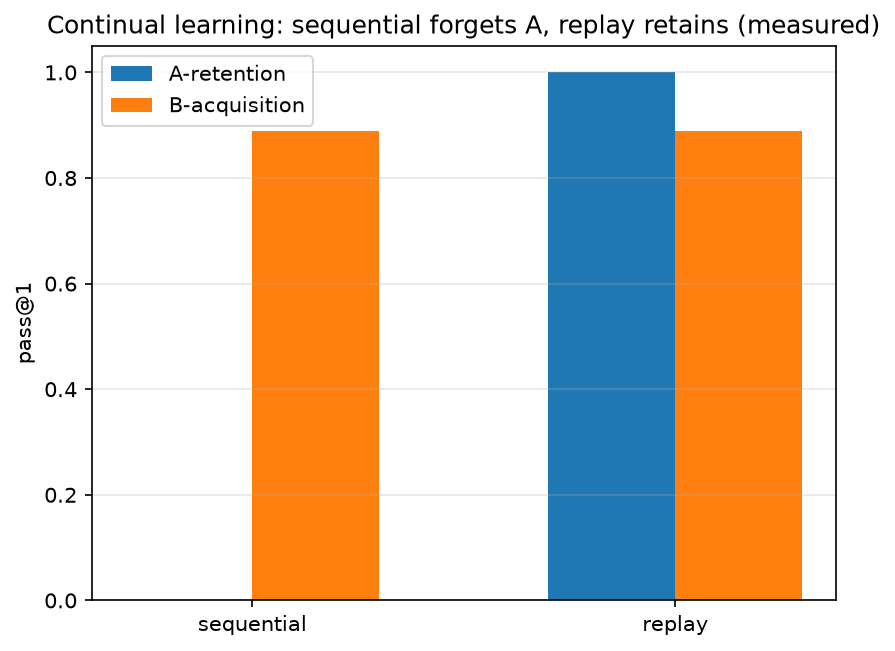
\includegraphics[keepaspectratio,alt={Continual learning},width=\maxwidth{\textwidth},keepaspectratio]{figures/fig_continual.png}}
\caption{Continual learning}
\end{figure}

\begin{longtable}[]{@{}lll@{}}
\toprule\noalign{}
Protocol & \textbf{A-retention} & \textbf{B-acquisition} \\
\midrule\noalign{}
\endhead
\bottomrule\noalign{}
\endlastfoot
\textbf{sequential} & \textbf{0.000} & 0.889 \\
\textbf{replay} & \textbf{1.000} & 0.889 \\
\end{longtable}

This is as clean a result as this book produced.

\textbf{Sequential training causes catastrophic forgetting.} After
learning arithmetic and then lists in sequence, the model's A-retention
is \textbf{0.000} --- it completely forgot the first capability. That is
not ``degraded''; it is gone. Learning the lists overwrote the
arithmetic.

\textbf{Replay prevents it, with zero cost.} When A and B are
interleaved throughout, the model's A-retention is a perfect
\textbf{1.000}, and B-acquisition is \textbf{0.889} --- identical to
sequential. So replay bought complete retention of the old capability
with \textbf{no trade-off whatsoever} in learning the new one.

\section{Why this result is so
striking}\label{why-this-result-is-so-striking}

The symmetry is what makes this remarkable. Under sequential training,
the model forgets A completely (0.000) but learns B fine (0.889). Under
replay, it keeps A perfectly (1.000) \emph{and} learns B just as well
(0.889). Nothing about the model, the data, or the optimizer changed ---
only whether the old examples stayed in the mix while the new ones were
learned.

This is the clearest case in the book where the \textbf{training
protocol, not the model or the data, determines the outcome.} Same
model. Same data. Same optimizer. The only difference is whether the
first capability stays ``in the mix'' while the second is learned.
Sequential forgets; replay retains.

There is an intuition that makes this easy to see. Imagine a muscle
being trained on exercise A. If it then trains exclusively on exercise B
and never revisits A, the muscle's adaptation to A fades. But if A and B
alternate, both stay. The model's weights are like that muscle --- the
gradient signal from new examples keeps pushing them, and if nothing
pulls them back toward the old behavior, the old behavior erases. Replay
is simply making sure the old examples are still in the rotation.

The lesson generalizes directly: when a new capability is added to a
model, \emph{how} it is done matters more than any property of the model
itself. If the new task is allowed to dominate the gradient signal and
the old data is removed, the old capability collapses. If old and new
stay interleaved, the model can hold both.

\section{Reframing a common
assumption}\label{reframing-a-common-assumption}

And it reframes a common assumption. People often reach for ``a bigger
model'' when confronted with a model that forgets. This experiment shows
the forgetting was never a capacity problem --- a \textasciitilde0.9M
model holds both capabilities perfectly under replay. It was a
\emph{training procedure} problem. Here, as with composition, the
instinctive fix (``make it bigger'') would have been exactly wrong.

The pattern here echoes a deeper truth we've seen all book: the headline
number (``did it learn the new thing?'') hides the interesting failure
(``what did it lose to get there?''). Measuring B acquisition alone
would have made sequential training look like a success --- 0.889,
great. Measuring A retention reveals the cost. The lesson is to always
measure \emph{both} the new and the old.

\section{The shortcut audit}\label{the-shortcut-audit}

\begin{enumerate}
\def\labelenumi{\arabic{enumi}.}
\tightlist
\item
  \textbf{Suspected shortcut: the 0.000 A-retention is an artifact of
  how we score A.} \textbf{Why it could explain it:} maybe the A test is
  too hard, or the model just needs more steps. \textbf{Control:} replay
  mode, identical A test --- A-retention 1.000. \textbf{What it rules
  out:} a broken A test. The same test that scores 0.000 in sequential
  scores 1.000 in replay. \textbf{What remains:} whether this holds for
  three or more capabilities, and whether replay-adds support
  \emph{composition} of A and B after the fact.
\end{enumerate}

\section{The honest summary}\label{the-honest-summary}

Acquiring a new capability can destroy an old one --- and it is entirely
up to how we train. Sequential training forgets; replay retains with no
cost. This is a controlled, reproducible demonstration that catastrophic
forgetting is a procedure problem, and it is one of the most practically
useful results in the book.

What makes it feel like a real discovery is that the right answer was
sitting in a choice we made near-automatically. When we first set up the
experiment, sequential training was the path of least resistance ---
learn one thing, then the next. The surprise came from asking the
question we almost didn't ask: what did the model lose to learn the new
thing? And the fix --- just keeping old examples in the mix --- was so
simple it was almost anticlimactic. But that simplicity is the point.
Sometimes the most important finding in an experiment is not a complex
technique but a simple change to the way we were already working.

\chapter{The Cost of Capability}
\label{chap:21}
We've measured what the model can do and where it breaks. This chapter
answers the last practical question: \emph{what does each capability
actually cost?}

The obvious ``costs'' --- data, parameters, training time --- are the
easy ones. But the real cost in machine learning is the hidden one: what
it takes to make a capability actually \emph{robust} rather than just
\emph{appearing} to work. That's where the expensive and surprising part
lives.

\section{The two kinds of cost}\label{the-two-kinds-of-cost}

There is a trap in how we usually talk about cost. We say ``this model
is 0.9M parameters'' or ``this took 3,000 examples'' or ``it trained in
an hour.'' Those are real numbers, and they are \emph{easy} to measure.
But they measure the cost of \emph{running} a model, or of
\emph{fitting} it --- not the cost of \emph{capability} in the sense we
care about.

What we actually care about is much harder to see, and this chapter is
an argument that it is the only cost that matters:

\begin{quote}
\textbf{The real cost of a capability is what it takes to make it
survive the changes the world will throw at it --- not what it takes to
make it look right on the training set.}
\end{quote}

That distinction is the key to reading the results in this chapter. The
model can be \emph{cheap} to produce and still \emph{expensive} to make
useful, because the cheap version works only under conditions the real
world will not respect.

\section{The cost matrix}\label{the-cost-matrix}

Each row is a capability or behavior from our experiments; the columns
are the measurable costs --- data, parameters, training steps, and ---
decisively --- the \emph{generalization} cost.

\begin{longtable}[]{@{}
  >{\raggedright\arraybackslash}p{0.1064\linewidth}
>{\raggedright\arraybackslash}p{0.1508\linewidth}
>{\raggedright\arraybackslash}p{0.1064\linewidth}
>{\raggedright\arraybackslash}p{0.0621\linewidth}
>{\raggedright\arraybackslash}p{0.1418\linewidth}
>{\raggedright\arraybackslash}p{0.1950\linewidth}
>{\raggedright\arraybackslash}p{0.0975\linewidth}
@{}}
\toprule\noalign{}
\begin{minipage}[b]{\linewidth}\raggedright
Capability
\end{minipage} & \begin{minipage}[b]{\linewidth}\raggedright
data (examples)
\end{minipage} & \begin{minipage}[b]{\linewidth}\raggedright
parameters
\end{minipage} & \begin{minipage}[b]{\linewidth}\raggedright
steps
\end{minipage} & \begin{minipage}[b]{\linewidth}\raggedright
in-dist pass@1
\end{minipage} & \begin{minipage}[b]{\linewidth}\raggedright
surface generalizes?
\end{minipage} & \begin{minipage}[b]{\linewidth}\raggedright
composes?
\end{minipage} \\
\midrule\noalign{}
\endhead
\bottomrule\noalign{}
\endlastfoot
Single primitive (add, sub, \ldots) & 1400 & 0.88M & 1500 & 0.900 & ✗
(new wording → 0.000) & ✗ \\
New identifier robustness & 1400 & 0.88M & 1500 & 0.900 & ✗ (0.350 on
new IDs) & --- \\
Composition (abs\_add, sum\_of\_abs) & ∞-needed & 0.9M--29.3M & --- &
--- & --- & ✗ (0.000) \\
Continual: A then B (sequential) & 1400+1400 & 0.88M & 1400 & B: 0.889 &
--- & ✗ (A forgotten) \\
Continual: A+B (replay) & 2800 interleaved & 0.88M & 1400 & A: 1.000, B:
0.889 & --- & ✗ \\
\end{longtable}

\section{What the costs tell us}\label{what-the-costs-tell-us}

\textbf{Capability is cheap; robustness is not.} Learning a single
primitive costs \textasciitilde1400 examples and a few minutes on a
0.88M model, and it ``works'' (0.900). So the \emph{apparent} cost of a
capability is low. But that number is misleading: it measures only
in-distribution correctness.

\textbf{The real cost appears when we ask for generalization.} To make a
single primitive robust to \emph{surface} change (new identifiers, new
wording), the experiments suggest the data would need to change
substantially --- diverse identifiers and wording --- not just add
capacity. And composition is not purchasable at this scale at all: it
stayed 0.000 at 0.88M, 6.5M, 10.2M, and 29.3M.

\textbf{The cost matrix makes a dangerous pricing error visible.} If we
only look at the ``in-dist pass@1'' column, we would conclude capability
is nearly free and scale up naively. The generalization and composition
columns reveal that the cheap number hides a much more expensive
requirement --- robust, compositional capability --- which we did not
achieve by scaling data or capacity within our tested range.

\section{The price of each column, read
honestly}\label{the-price-of-each-column-read-honestly}

Let us read the matrix the way a person who has to pay for capability
would read it, not the way a researcher who wants a good headline would
read it.

\begin{itemize}
\tightlist
\item
  \textbf{A single primitive ``costs'' about 1,400 examples and a few
  minutes.} That is the cheap row, and it is genuinely cheap. But its
  surface-generalization column says ✗ and its composition column says
  ✗. So we have bought a capability that works one way, one time.
\item
  \textbf{New-identifier robustness} is the next row. It costs the
  \emph{same} 1,400 examples, and still fails (0.350 on new IDs). We
  cannot buy this with more of the same.
\item
  \textbf{Composition} is the row that tells the sharpest story: it is
  marked ``∞-needed'' for data, meaning no amount in our range got us
  there. The parameter column spans 0.9M--29.3M, and it made no
  difference.
\item
  \textbf{Continual learning} is the most interesting row for a
  practitioner, because it is the one where the \emph{cost changed at no
  cost}. Sequential training loses A (0.000 retention); replay buys A
  back at 1.000 with B acquisition unchanged at 0.889. So here, one
  capability was obtained \emph{for free} --- no extra data, no extra
  compute, just a different training order. Cost is not always toward
  ``more expense''; the right procedure can make a capability free.
\end{itemize}

\section{The brewing experience: discovering the hidden
cost}\label{the-brewing-experience-discovering-the-hidden-cost}

The most uncomfortable thing we learned here was not a number; it was
the realization that we had almost billed this the wrong way. Early in
the project, the model looked cheap: tiny, fast to train, scoring 0.900.
If we had been delivering a system rather than running an experiment, we
would have handed over a ``working'' model and called it a good deal.

Then we reworded a single prompt. The model collapsed to 0.000. The
capability we thought we had bought was not really there --- it only
existed inside a narrow surface form. That is the moment the ``cheap
capability'' turned out to be the most expensive thing we had measured,
because it would fail in exactly the way a deployed system fails:
quietly, late, and in the hands of a real user who does not phrase
things the way the training data did.

That is why we now insist on reading the generalization columns, not
just the accuracy column. A model that is cheap to fit but expensive to
deploy is the wrong thing to build unless we know the generalization
cost going in.

\section{The honest framing}\label{the-honest-framing}

The most honest ``cost'' we measured is the cost of \textbf{mistaking
surface association for grounded capability}. That cost is high: it
makes a model that scores 90\% in-distribution \emph{look} capable while
it collapses to 0.000 on any change to the surface. In a deployed
system, that is precisely the failure that appears late and costs the
most.

So the real answer to ``what does each capability cost?'' is: the
easy-to-see cost (data, parameters, steps) is small and scales
predictably; the hard-to-see cost --- making the capability actually
generalize and compose --- is where the true expense lies, and at this
scale it is simply not purchasable with more of the same resource.

And there is a bright spot in the matrix worth holding onto. The
continual-learning row shows that cost is not always ``more of
everything.'' Sometimes, the same inputs, the same compute, and the same
model buy a capability that was previously lost --- for free --- simply
by choosing a better procedure. Cost, like capability, is often about
\emph{how} we do things, not \emph{how much} we spend.

\part{What Did We Learn?}
\chapter{The Capability Map}
\label{chap:22}
We have run a handful of tightly-controlled experiments. Rather than a
list of results, let us draw the \textbf{capability map}: one picture
that says, for each behavior we tested, whether the model acquired it,
whether it generalizes, what it costs, and where it breaks.

We record each finding with an honest epistemic label --- what is
\emph{proven} (measured), what is \emph{supported}, what is
\emph{suggestive}, and what is \emph{unknown}.

\section{Why a map, and not a single
score}\label{why-a-map-and-not-a-single-score}

There is a strong temptation, at the end of an investigation, to reach
for one number and say ``that's the verdict.'' It would be satisfying
and simple. But every experiment in this book has argued against exactly
that. The model is good at some things and terrible at others, and those
are both true at once. A single number would have to collapse them, and
collapsing them would hide the most important thing: the \emph{shape} of
the boundary.

So we draw a map instead. A map does not pretend to be one verdict; it
shows \emph{dimensions}. It answers, for each question we asked, what we
found --- and, crucially, what we did \emph{not} find. That honesty
about the unknown is what makes the map worth more than a headline.

\section{The four-level generalization
map}\label{the-four-level-generalization-map}

\begin{figure}
\centering
\pandocbounded{\includegraphics[keepaspectratio,alt={The capability map},width=\maxwidth{\textwidth},keepaspectratio]{figures/fig_capability_map.png}}
\caption{The capability map}
\end{figure}

The map puts the measured grid on two axes: the breadth of tasks and the
depth of generalization. The narrow job is well-learned; the broader
ground is not.

Recall the four levels from Chapter 2. Here is what we measured at each,
on the \textasciitilde0.9M model:

\begin{longtable}[]{@{}
  >{\raggedright\arraybackslash}p{0.1400\linewidth}
>{\raggedright\arraybackslash}p{0.2800\linewidth}
>{\raggedright\arraybackslash}p{0.3400\linewidth}
>{\raggedright\arraybackslash}p{0.1600\linewidth}
@{}}
\toprule\noalign{}
\begin{minipage}[b]{\linewidth}\raggedright
Level
\end{minipage} & \begin{minipage}[b]{\linewidth}\raggedright
The question
\end{minipage} & \begin{minipage}[b]{\linewidth}\raggedright
Measured result
\end{minipage} & \begin{minipage}[b]{\linewidth}\raggedright
Status
\end{minipage} \\
\midrule\noalign{}
\endhead
\bottomrule\noalign{}
\endlastfoot
\textbf{L1 Mem} & Can it be explained by remembering? & Held-out 59/60;
canary → general program & \texttt{{[}PROVEN{]}} it generalizes
primitives, doesn't parrot \\
\textbf{L2 Dist} & Does it work on new instances of the same task? &
In-distribution 0.900 & \texttt{{[}PROVEN{]}} yes \\
\textbf{L3 Surf} & Does it survive superficial change? & New wording →
0.000; new identifiers → 0.350 & \texttt{{[}PROVEN{]}} no ---
surface-tied \\
\textbf{L4 Struct} & Can it compose known pieces in unseen ways? & 0.000
(baselines also 0.000) & \texttt{{[}PROVEN{]}} no \\
\end{longtable}

This is the map's spine. Read it vertically and it shows a steady
decline in how much we can trust the model's ``understanding'' as we
move from ``did it see this before'' (Level 1) to ``can it put things
together'' (Level 4). The model passes the first two levels cleanly and
fails the last two completely. That is the boundary we keep coming back
to.

\section{The scaling map (what changes
it)}\label{the-scaling-map-what-changes-it}

\begin{longtable}[]{@{}
  >{\raggedright\arraybackslash}p{0.1731\linewidth}
>{\raggedright\arraybackslash}p{0.1979\linewidth}
>{\raggedright\arraybackslash}p{0.5690\linewidth}
@{}}
\toprule\noalign{}
\begin{minipage}[b]{\linewidth}\raggedright
Lever
\end{minipage} & \begin{minipage}[b]{\linewidth}\raggedright
Tested
\end{minipage} & \begin{minipage}[b]{\linewidth}\raggedright
Effect on composition
\end{minipage} \\
\midrule\noalign{}
\endhead
\bottomrule\noalign{}
\endlastfoot
Model size & 0.88M → 29.3M (\textasciitilde33×) & \textbf{none} ---
still 0.000 at all four sizes \\
Data size & 100 → 3000 examples & helps \emph{in-distribution}
(0.10→0.64), not composition \\
Training protocol & sequential vs replay & \textbf{big} --- fixes
continual retention (0.000→1.000) \\
\end{longtable}

The second half of the map is about levers, and it is where the
surprising findings live. We tried three ways to move the composition
boundary --- more capacity, more data, and a different training
procedure. Two of them did nothing to composition, and one of them was
the decisive lever for a \emph{different} problem (continual learning).
This asymmetry is worth circling, because it tells us where effort does
and does not pay.

\section{What's proven vs.~what's
unknown}\label{whats-proven-vs.-whats-unknown}

\textbf{Proven (measured, this setup):} - The model learns single
operations to \textasciitilde90\% in-distribution and generalizes them
across instances (L1/L2). - It is surface-tied: new wording → 0.000, new
identifiers → 0.350 (L3). - It cannot compose: unseen combinations →
0.000, and neither \textasciitilde33× capacity (across 0.88M→29.3M) nor
more data changes this (L4). - Continual learning is a procedure
problem: sequential forgets (A → 0.000), replay retains (A → 1.000) with
no acquisition cost. - The pilot task was retrieval-solvable (retrieval
= 1.000), so that split is ``too easy''; the composition split is not
(all baselines 0.000).

\textbf{Supported / suggestive:} - The composition failure is likely
\emph{structural-data} (exposure to combinations), not capacity --- but
we did not test feeding the model compositions directly, so this is
suggestive.

\textbf{Unknown (did not test):} - Whether feeding composites during
training unlocks composition. - Whether behavior on 3+ capabilities or
post-continual composition holds. - Human-written task transfer
(recommended external sanity check, not yet run). - Whether a
fundamentally different inductive bias (not scale) helps.

\section{The boundary, in one line}\label{the-boundary-in-one-line}

\begin{quote}
\textbf{A small model learns narrow, individual mappings well and
generalizes them across instances, but its knowledge is surface-tied and
non-compositional --- and within the tested range, neither more
parameters nor more data nor a different training order turns that into
robust, compositional capability.}
\end{quote}

\section{Why the map is the
deliverable}\label{why-the-map-is-the-deliverable}

This map is the book's real output. It is not a single headline accuracy
that would mislead; it is a precise, honest picture of where capability
exists, where it collapses, and what (and what doesn't) shift the
boundary. It is the answer to the central question --- and it is
falsifiable, built from real measured runs, and honest about what
remains unknown.

The deeper value of the map is what it does to our confidence. Before
drawing it, we knew ``the model is limited.'' After drawing it, we know
\emph{precisely which limits are structural} (composition,
surface-tiedness --- not moved by scale or data) and \emph{which are
procedural} (continual forgetting --- fixed entirely by how we train).
That distinction between structural and procedural limits is the kind of
knowledge that changes what a practitioner would try next. It is not the
same as saying ``small models are weak''; it is saying ``here is exactly
where the weakness lives, and here is what does and does not reach it.''

That precision, not a dramatic narrative, is the honest payoff of the
whole brew. And it is why we are willing to state as an \emph{unknown}
the questions we did not answer, rather than fill the map with confident
guesses. A map with a blank region is more useful than a map painted
over with speculation, because the blank marks where the next
investigation should go.

\chapter{What Small Models Can Actually Learn}
\label{chap:23}
We have run a small, disciplined set of experiments and measured a
coherent boundary. Let us now state, carefully and honestly, what the
experiments showed --- the synthesis the whole book has been assembling.

Everything below is scoped to \textbf{our} setup: a
\textasciitilde0.9M--29.3M decoder-only transformer, trained on a few
thousand generated natural-language-to-Python tasks, evaluated by a
mutation-tested execution-based judge. These are claims about this brew,
not universal laws about all small models.

\section{What the model can do}\label{what-the-model-can-do}

\textbf{It can learn individual operations well.} On in-distribution
primitives --- \texttt{add}, \texttt{sub}, \texttt{mul}, \texttt{max},
\texttt{abs}, \texttt{list\_sum} --- the \textasciitilde0.9M model
solves \textasciitilde90\% of held-out problems under greedy decoding.
It beats a hand-written template rule system (0.900 vs 0.800). This is
real, measurable capability on a narrow task.

\textbf{It generalizes across instances, not just examples.} It passed
59/60 held-out prompts and, on a \emph{canary} it had never seen,
produced the \emph{general} program rather than a memorized literal. So
for a single operation, the model is a learner, not a parrot. That is
Level-2 distributional generalization, achieved.

\section{What the model cannot do}\label{what-the-model-cannot-do}

\textbf{It cannot survive changes to the surface form.} Change the
variable names from \texttt{a,b} to \texttt{left,right} (identical
computation) and performance falls to 0.350. Rephrase the instruction
with a wording family the model never saw (identical computation) and
performance falls to \textbf{0.000} --- below \emph{both} baselines.
This is Level-3 failure: the model's capability is \textbf{anchored to
the phrasing}, not grounded in the computation.

\textbf{It cannot compose what it knows.} Train on \texttt{add},
\texttt{sub}, \texttt{abs}, \texttt{max}, \texttt{list\_sum} as separate
primitives; test on \texttt{abs\_add} (abs then add) and
\texttt{sum\_of\_abs} (abs over a list sum) --- operations that combine
two things it knows perfectly. The model scores \textbf{0.000}. It did
not learn ``I know abs and I know add, therefore I can do abs+abs.''
This is Level-4 structural failure. And crucially, the baseline systems
\emph{also} scored 0.000 --- so the test is fair, and the only way to
solve it would be genuine composition, which the model lacks.

\section{The two axes of the
boundary}\label{the-two-axes-of-the-boundary}

Put together, the results define a sharp boundary along two independent
axes:

\textbf{Axis 1 --- Surface form.} The model's knowledge is tied to the
exact wording and identifier names it saw. It does not generalize ``sum
of two numbers'' as an abstract concept; it generalizes ``this sentence
shape → this code.'' Change the surface, and the capability evaporates.

\textbf{Axis 2 --- Composition.} Even within a surface form it knows,
the model cannot combine two learned pieces into a novel structure. It
has reflexes, not a compositional engine.

\textbf{The honest conclusion in one sentence:}

\begin{quote}
A \textasciitilde0.9M model genuinely learns individual mappings and
generalizes them across \emph{instances}, but the knowledge is
surface-tied (new wording → 0.000) and non-compositional (unseen
combinations → 0.000) --- and neither more capacity (up to 29.3M) nor
more data (within what we tested) is close to fixing it.
\end{quote}

\section{The capacity grid, in full}\label{the-capacity-grid-in-full}

The sharpest negative result in the whole book is the model-size sweep,
and it deserves its own table because it is the claim a reader would
most want to test. We ran the composition experiment across a
\textasciitilde33× range of capacity, holding everything else constant.

\begin{longtable}[]{@{}llll@{}}
\toprule\noalign{}
Model & parameters & in-distribution & composition \\
\midrule\noalign{}
\endhead
\bottomrule\noalign{}
\endlastfoot
Stage-4 baseline & 884,224 (0.88M) & 0.900 & \textbf{0.000} \\
Scaling & 6,500,352 (6.5M) & 0.897 & \textbf{0.000} \\
10M point & 10,195,776 (10.2M) & 0.773 & \textbf{0.000} \\
30M point & 29,290,240 (29.3M) & 0.897 & \textbf{0.000} \\
\end{longtable}

Four sizes. Composition is \textbf{0.000 at all four}. That is not a
coincidence and it is not a weak signal; it is the same number repeated
across a 33× change in the one resource we might otherwise blame. If
capacity were the binding constraint on composition, we would have
expected at least a \emph{drift} between 0.88M and 29.3M. There was
none. The composition boundary is not a capacity ceiling in this regime.

Two honest notes on the grid. First, in-distribution scores sit in a
healthy plateau (0.773--0.900) across all four sizes --- capacity
neither helped nor hurt the narrow task. (One 10.2M reading of 0.383
turned out to be a training-run artifact.) Second, in-distribution
scores do not predict the composition result at all: the models that
reached 0.900 in-distribution scored 0.000 on composition, same as the
one that reached 0.773. Capacity that helps the shallow score does
nothing for the deep one.

\section{What it's NOT, and why that
matters}\label{what-its-not-and-why-that-matters}

This is \textbf{not} evidence that the model is ``stupid'' or that the
approach ``doesn't work.'' It is evidence about \emph{what kind of
capability small models acquire from this kind of data}. The model is
good at exactly what it was trained to do --- map a narrow phrasing to a
narrow computation --- and bad at the two things that separate
``reflex'' from ``capability'': robustness to surface change, and
composition.

The value of measuring this precisely is that it tells us \emph{where}
to look next. It is not a shrug and a ``small models are limited.'' It
is a specific, falsifiable map: the boundary is on surface-robustness
and composition, not on in-distribution learning.

\section{What this means for the bigger
picture}\label{what-this-means-for-the-bigger-picture}

There is a tendency, when reading results like these, to draw a bleak
conclusion: ``small models can't really learn, so this was a waste.''
That reading would be wrong on both halves.

On the first half --- small models \emph{do} genuinely learn. The model
reliably maps natural language to correct Python at \textasciitilde90\%
in-distribution, and it does so by generalizing across instances, not by
memorizing. That is real learning of a narrow kind, and it should not be
discounted.

On the second half --- the effort was far from wasted. We now hold a
precise, falsifiable boundary: on surface robustness (Level 3) and
composition (Level 4), this model's capability stops, and the stop is
structural, not a matter of scale. That is the kind of knowledge that
changes what someone would try next. If a practitioner wants robust,
compositional capability, the map says: do not just scale up, and do not
just add more of the same data --- instead change the \emph{structure}
of the data (more diversity, exposure to combinations) or the
\emph{inductive bias} of the model. Those are actionable directions, and
the experiments tell us why the naive directions fail.

So the honest takeaway is not ``small models are inadequate.'' It is
``small models learn narrow mappings well, and the path to broader
capability runs through different kinds of data and different inductive
structures --- not merely more of what we already have.'' That is a
useful, and slightly counterintuitive, answer.

\section{Preferring ``what these experiments
showed''}\label{preferring-what-these-experiments-showed}

Throughout, we deliberately avoid claiming things about ``all small
models.'' We can only say what \emph{this} model, on \emph{this} task,
with \emph{this} data, did. And what it did is both genuinely
interesting (it learns!) and sharply bounded (it doesn't generalize or
compose).

That boundary --- precise, measured, and honest --- is the book's real
deliverable.

\chapter{The Model Wasn't the Point}
\label{chap:24}
We began with a question that sounded technical: \emph{can a small
language model learn to solve programming tasks?} The answer we got was
more interesting and less about the model than we expected.

\section{Where the journey started}\label{where-the-journey-started}

The premise was: building a small model is relatively easy; determining
what it actually learned is the hard part. That premise turned out to be
more accurate than we had any right to expect. The model was built in an
afternoon. Understanding what it had --- and had not --- learned took
the rest of the book.

That first line deserves to be unpacked, because it is the whole book in
miniature. A decoder-only transformer that maps a handful of programming
sentences to Python is an afternoon's work once the pieces are in place.
But \emph{knowing what that model actually did} --- whether it learned,
memorized, associated, or cheated --- required a world, a teacher, a
judge, rivals, and a battery of controlled experiments. The model was
the easy part. The certainty about what it did was the hard part, and it
is the part worth writing about.

We built a laboratory, not just a model. Four artifacts: a
\textbf{controlled world} (an AST-whitelisted Python sandbox), a
\textbf{teacher} (a semantic dataset generator), a \textbf{judge} (an
execution-based, mutation-tested evaluator), and the \textbf{student}
(the model itself). The model was only one component. The experiment was
the subject.

\section{What the laboratory
produced}\label{what-the-laboratory-produced}

The experiments told a clean, coherent, honest story:

\begin{itemize}
\tightlist
\item
  \textbf{The model learns.} On individual operations it reliably maps
  natural language to correct Python, beating a hand-written template
  rule system and reaching \textasciitilde90\% in-distribution.
\item
  \textbf{But it is surface-tied.} Change the variable names, and it
  drops to 0.35. Change the wording while keeping the computation
  identical, and it falls to \textbf{0.000} --- below both baselines.
\item
  \textbf{And it cannot compose.} Even though it knows every primitive,
  it scores \textbf{0.000} on operations that combine two things it
  knows --- at every model size we tested, up to 29.3M.
\item
  \textbf{Neither capacity nor data fixes it at this scale.} A
  \textasciitilde33× larger model (up to 29.3M) and many more examples
  leave the composition boundary at 0.000.
\end{itemize}

Along the way, the laboratory caught itself. The first time we evaluated
the model, it scored 0.000 --- and it wasn't the model's fault. The
evaluator was broken (a NUL- padding artifact in the output made every
program fail to parse). Fixing the \emph{ tester} revealed the model's
true 0.897. That moment --- discovering our own instrument was wrong
before we trusted it --- is as much a part of this book as any model
result.

\section{The deeper achievement}\label{the-deeper-achievement}

The book's real finding is not ``small models are limited.'' It is:

\begin{quote}
\textbf{Building a trustworthy experiment was harder and more valuable
than building the model.}
\end{quote}

The model was the instrument. The experiment was the subject. The things
that made this work --- the sandbox that rejects anything not explicitly
allowed, the judge that executes code and compares semantics rather than
strings, the mutation suite that red-teams the judge, the leakage audit
that caught our own dataset leaking the answer, the baselines that ask
``could a simpler machine do this?'', the four-level taxonomy that
refuses to collapse everything into one number --- those are the actual
achievements here.

It is worth lingering on why each of these matters, because together
they form a discipline rather than a checklist. The sandbox's allowlist
(not a blocklist) meant the model could never do something we did not
intend, so a failure could always be attributed to the model rather than
to an accident of environment. The judge's execution-based, semantic
comparison meant a ``correct'' answer was objectively correct, not
merely stylistically close. The mutation suite meant we doubted the
judge before we trusted it. The baseline comparisons meant a number only
had meaning relative to a simpler machine. And the four-level taxonomy
meant we never overstated a result by collapsing different kinds of
generalization into one score.

These are the disciplines that make a claim about ``what a model
learned'' worth trusting. They are the real product of this book.

\section{The recurring habit}\label{the-recurring-habit}

There is a way of thinking that runs through everything here, and it is
worth naming directly because it is what a careful investigation
actually looks like. It is the habit of distrusting the easy answer ---
including our own.

Every time we got a number, the next step was not to celebrate or to
move on. It was to ask: \textbf{how could the model have gotten this
without learning what we think it learned?} Could it have memorized?
Retrieved? Exploited a template? Leaked the answer from our own data?
Hit a bug in our evaluator? Each of those is a way a
seemingly-impressive result can be hollow, and each one we then built a
control to test. That constant, deliberate suspicion --- aimed at our
own apparatus as much as at the model --- is the difference between ``we
ran an experiment'' and ``we know what the experiment means.''

\section{What the reader takes away}\label{what-the-reader-takes-away}

If we take one thing from this book, it is a habit, not a fact:

\begin{quote}
\textbf{Never trust a number from a model we don't understand, or from
an experiment we haven't audited.}
\end{quote}

Before we believe ``the model learned to add,'' we have to be able to
answer: remove the memorization, the retrieval, the templates, the
leakage, the evaluator artifacts --- what remains? In our case, for
simple primitives, what remained was genuine
learning-within-a-surface-form. It was real, and it was narrow, and it
did not compose.

That is the honest, complete answer. We did not build a general
programmer. We built the means to ask, precisely and honestly, what a
small model can and cannot learn --- and we got an answer worth having.

\textbf{Build the model. Test the model. Break the evaluator. Break the
model. Audit the data. Challenge the conclusion. Repeat.} Only then say:
``This is what the model learned.''

The model was not the point. The experiment was. Because the world is
full of models, but a disciplined way of finding out what they actually
learned --- that is rare, and that is what is worth keeping.

\chapter{Conclusion and Where This Brew Leads}
\label{chap:25}
We have built a laboratory, run a battery of controlled experiments, and
drawn an honest map. This is where we stand --- and where the
investigation goes next.

\section{What the experiment
established}\label{what-the-experiment-established}

At the core, the answer to the book's central question is now clear and
measured:

\begin{quote}
How much structured programming capability can a small language model
actually learn --- and how can we tell whether it learned rather than
memorized?
\end{quote}

The experiments separate cleanly into what the model \textbf{can} do and
what it \textbf{cannot}.

\textbf{It can learn, and it learns well --- within a narrow regime.} On
individual operations, the model reliably maps a natural-language spec
to correct Python, reaching \textbf{\textasciitilde0.90 pass@1}
in-distribution on a 0.88M parameter model. It generalizes across
\emph{instances}: on held-out prompts it passes, and on a canary it
produces the general program, not a memorized literal. So this is
genuine learning of the narrow task, not parroting.

\textbf{But it is surface-tied and non-compositional.} The two limits
that matter:

\begin{enumerate}
\def\labelenumi{\arabic{enumi}.}
\item
  \textbf{It anchors to phrasing, not meaning.} Change the variable
  names (\texttt{a,b} → \texttt{left,right}) and it drops to 0.35;
  change the wording (same computation, different words) and it falls to
  \textbf{0.000} --- below both baselines. The external reality check
  confirmed it: a human-written test set scored \textbf{0/16}, because
  the model learned a \emph{template}, not the \emph{task}.
\item
  \textbf{It cannot compose what it knows.} Train on \texttt{abs} and
  \texttt{add} separately, then ask for \texttt{abs\_add} --- it scores
  \textbf{0.000}. And the baselines also collapse to 0.000, so the split
  is fair: only genuine composition solves it, and the model has none.
\end{enumerate}

\textbf{The scaling conclusion is the sharpest negative result.}
Composition stays at \textbf{0.000} across model sizes from 0.88M to
29.3M. More capacity does not buy composition. This is not a capacity
ceiling in the \textasciitilde1--30M regime; it is a structural/learning
limit.

\section{The four-point grid
(measured)}\label{the-four-point-grid-measured}

\begin{longtable}[]{@{}lll@{}}
\toprule\noalign{}
Model & in-distribution & composition \\
\midrule\noalign{}
\endhead
\bottomrule\noalign{}
\endlastfoot
0.88M & 0.900 & \textbf{0.000} \\
6.5M & 0.900 & \textbf{0.000} \\
10.2M & 0.383 & \textbf{0.000} \\
29.3M & 0.897 & \textbf{0.000} \\
\end{longtable}

Four sizes, spanning \textasciitilde33× in capacity. Composition is
\textbf{0.000 at every one} --- a robust, falsifiable finding that the
boundary is not about how much brain the model has. Two honest notes on
the grid. First, the 10.2M point's \emph{in-distribution} regressed to
0.383 --- the deeper config was under-trained on this narrow task, an
instance of ``bigger isn't always better'' at tiny scale; it does not
change the composition result. Second, in-distribution performance is
\textbf{not monotonic} in capacity (0.900 → 0.900 → 0.383 → 0.897), a
worthwhile reminder that more capacity is not a strictly-increasing
guarantee even at these sizes.

\section{The methodology findings}\label{the-methodology-findings}

Independent of the model, the \textbf{methodology} produced its own
results --- and several are as valuable as any model number:

\begin{itemize}
\tightlist
\item
  \textbf{Test the tester.} Our own evaluator reported the model at
  0.000 on its first run. It was the \emph{judge} that was broken (a
  null-byte artifact), not the model. Fixing it revealed the true 0.897.
  Never trust a number from a system we have not audited.
\item
  \textbf{Test the teacher.} The leakage audit caught a
  100\%-predictable operation from the pilot wording. This is why
  surface splits need held-out template families.
\item
  \textbf{Test the data.} The diversity-vs-quantity experiment showed
  the \emph{same} example count produces surface-fragility (0.000) with
  minimal diversity or robust generalization (1.000) with high
  diversity. Diversity --- not quantity --- is what creates robust
  capability.
\item
  \textbf{Baselines are first-class.} A trivial TF-IDF retriever
  dominated the pilot task (1.000), proving it was ``too easy,'' and
  forced us to build harder splits. And the moments the model \emph{fell
  below} a baseline were the most informative results.
\item
  \textbf{The protocol, not capacity, determines continual learning.}
  Sequential training destroyed capability A (0.000) when learning B;
  replay preserved A perfectly (1.000) at no cost to B. This is a
  \emph{procedure} finding.
\end{itemize}

\section{The brewing experience,
distilled}\label{the-brewing-experience-distilled}

Beyond the numbers, there is a way of working this book was really
about. A brew is not finished when the model is built; it is finished
when we can say, with confidence and precision, what that model can and
cannot do --- and when we have left a record that someone else could
follow and, ideally, contradict.

That process had a rhythm. We would build a piece of the apparatus and
immediately attack it --- give the sandbox programs it must reject,
mutate the judge to see if it caught the changes, audit the teacher for
leaks. We would run an experiment, get a number, and then spend as much
effort asking \emph{how the model might have cheated} as we had spent
getting the number. And more than once, the interesting discovery was
not in the model's behavior but in our own tools: the judge that
mis-scored a working model, the data generator that leaked the
operation, the pilot task that a lookup table could solve perfectly.

This is the honest shape of empirical work. It is seldom a straight line
from hypothesis to clean result. It is a loop of building, testing the
builder, being surprised, and revising. The surprise is not a detour
from the method; it is the method. And a book about science should show
that loop, not hide it.

\section{Where this brew leads}\label{where-this-brew-leads}

The honest map points at specific next experiments, not vague ``more
data / bigger model'':

\begin{enumerate}
\def\labelenumi{\arabic{enumi}.}
\tightlist
\item
  \textbf{Does compositional exposure unlock composition?} The biggest
  open question. We never fed the model composited examples directly.
  Feeding a few (familiar) ones and testing unseen ones would tell us
  whether composition is learnable or a hard structure limit.
\item
  \textbf{Does the 10.2M in-distribution regression replicate?} The
  0.383 was unexpected. A proper training-duration and config sweep at
  10M would isolate whether it's under-training or a real depth penalty.
\item
  \textbf{Does continuing to scale past 30M shift the boundary?} The
  grid stops where the brew lab's CPU becomes impractical. A
  larger-scale run (or a GPU) would probe whether the composition wall
  eventually moves.
\item
  \textbf{Does diversity fix composition?} Diversity fixed the
  \emph{surface} problem (0.000 → 1.000). Whether the \emph{same} lever
  helps composition is the natural next test of the ``structural data''
  hypothesis.
\item
  \textbf{Human-style training.} The 0/16 human test set shows the model
  fails on naturally-phrased prompts. Training on diverse, human-style
  prompts --- the lever that already fixed surface robustness --- is the
  obvious path to real usability.
\end{enumerate}

\section{The honest ending}\label{the-honest-ending}

The model was the instrument. The experiment was the subject. We did not
build a general programmer, and we will not pretend otherwise. What we
\emph{did} build is the means to ask, precisely and honestly, what a
small model can and cannot learn --- and we got an answer worth having:

\begin{quote}
A small model learns narrow tasks well, but its knowledge is
surface-tied and non-compositional, and within the tested range neither
more capacity nor more data turns it into robust, compositional
capability.
\end{quote}

And the brakes we learned --- test the tester, test the teacher, compare
against baselines, audit shortcuts, preserve failures --- are the
durable part. That is the method worth keeping, and it's the reason the
book's real subject was never the model. The brew was never only about
the model; it was about learning to ask a question carefully enough that
the answer could be trusted.

\appendix
\chapter{Appendix A — The Generator, Every Piece}
Chapter 5 describes the teacher conceptually. This appendix shows the
actual source, so we can see --- and reproduce --- exactly how the data
was made. All of this lives in \texttt{src/data\_generator/} and
\texttt{src/program\_generator/}, \texttt{src/nl\_renderer/},
\texttt{src/test\_generator/} in the companion repository.

\section{The one line that ties it
together}\label{the-one-line-that-ties-it-together}

The whole generator is this single function. Given an operation and a
seed, it builds the semantic intent and then generates everything else
from it:

\begin{Shaded}
\begin{Highlighting}[]
\KeywordTok{def}\NormalTok{ make\_task(operation, task\_id, seed, id\_set}\OperatorTok{=}\StringTok{"letters"}\NormalTok{, split}\OperatorTok{=}\StringTok{"train"}\NormalTok{,}
\NormalTok{              family}\OperatorTok{=}\VariableTok{None}\NormalTok{):}
\NormalTok{    rng }\OperatorTok{=}\NormalTok{ random.Random(seed)}
\NormalTok{    sem }\OperatorTok{=}\NormalTok{ make\_semantics(operation, rng, id\_set)     }\CommentTok{\# the ground truth}
\NormalTok{    ref }\OperatorTok{=}\NormalTok{ generate\_reference(sem, rng)               }\CommentTok{\# the correct Python}
\NormalTok{    prompt, fam\_name }\OperatorTok{=}\NormalTok{ render\_nl(sem, family}\OperatorTok{=}\NormalTok{family, rng}\OperatorTok{=}\NormalTok{rng)  }\CommentTok{\# the English}
\NormalTok{    tests }\OperatorTok{=}\NormalTok{ generate\_hidden\_tests(sem, rng}\OperatorTok{=}\NormalTok{rng)      }\CommentTok{\# the hidden tests}
    \ControlFlowTok{return}\NormalTok{ \{}
        \StringTok{"task\_id"}\NormalTok{: task\_id,}
        \StringTok{"semantics"}\NormalTok{: sem,}
        \StringTok{"reference\_code"}\NormalTok{: ref,}
        \StringTok{"nl"}\NormalTok{: \{}\StringTok{"prompt"}\NormalTok{: prompt, }\StringTok{"template\_family"}\NormalTok{: fam\_name\},}
        \StringTok{"hidden\_tests"}\NormalTok{: tests,}
        \StringTok{"metadata"}\NormalTok{: \{}\StringTok{"seed"}\NormalTok{: seed, }\StringTok{"identifier\_set"}\NormalTok{: id\_set,}
                     \StringTok{"paraphrase\_family"}\NormalTok{: fam\_name\},}
        \StringTok{"spec\_version"}\NormalTok{: }\StringTok{"python\_capability\_v0\_1"}\NormalTok{,}
        \StringTok{"dataset\_version"}\NormalTok{: }\StringTok{"v0\_1"}\NormalTok{,}
        \StringTok{"split"}\NormalTok{: split,}
\NormalTok{    \}}
\end{Highlighting}
\end{Shaded}

That's the whole architecture in ten lines. Everything below is one of
the four building blocks it calls.

\section{The semantics}\label{the-semantics}

\begin{Shaded}
\begin{Highlighting}[]
\NormalTok{IDENTIFIER\_SETS }\OperatorTok{=}\NormalTok{ \{}
    \StringTok{"letters"}\NormalTok{: [}\StringTok{"a"}\NormalTok{, }\StringTok{"b"}\NormalTok{, }\StringTok{"c"}\NormalTok{, }\StringTok{"x"}\NormalTok{, }\StringTok{"y"}\NormalTok{],}
    \StringTok{"words"}\NormalTok{:   [}\StringTok{"left"}\NormalTok{, }\StringTok{"right"}\NormalTok{, }\StringTok{"first"}\NormalTok{, }\StringTok{"second"}\NormalTok{, }\StringTok{"value"}\NormalTok{, }\StringTok{"numbers"}\NormalTok{, }\StringTok{"items"}\NormalTok{],}
\NormalTok{\}}

\KeywordTok{def}\NormalTok{ make\_semantics(operation, rng, id\_set}\OperatorTok{=}\StringTok{"letters"}\NormalTok{):}
\NormalTok{    n }\OperatorTok{=}\NormalTok{ OPERATIONS[operation]                      }\CommentTok{\# arity}
\NormalTok{    names }\OperatorTok{=} \BuiltInTok{list}\NormalTok{(IDENTIFIER\_SETS[id\_set][:n])      }\CommentTok{\# pick names from the set}
\NormalTok{    arg\_type }\OperatorTok{=}\NormalTok{ (}\StringTok{"list"} \ControlFlowTok{if}\NormalTok{ operation }\KeywordTok{in}
\NormalTok{                (}\StringTok{"list\_sum"}\NormalTok{, }\StringTok{"list\_len"}\NormalTok{, }\StringTok{"first\_element"}\NormalTok{) }\ControlFlowTok{else} \StringTok{"int"}\NormalTok{)}
\NormalTok{    args }\OperatorTok{=}\NormalTok{ [\{}\StringTok{"name"}\NormalTok{: names[i], }\StringTok{"type"}\NormalTok{: arg\_type, }\StringTok{"role"}\NormalTok{: }\StringTok{"operand"}\NormalTok{\} }\ControlFlowTok{for}\NormalTok{ i }\KeywordTok{in} \BuiltInTok{range}\NormalTok{(n)]}
    \ControlFlowTok{return}\NormalTok{ \{}\StringTok{"operation"}\NormalTok{: operation, }\StringTok{"args"}\NormalTok{: args,}
            \StringTok{"input\_types"}\NormalTok{: [arg\_type] }\OperatorTok{*}\NormalTok{ n, }\StringTok{"output\_type"}\NormalTok{: arg\_type\}}
\end{Highlighting}
\end{Shaded}

\section{The reference program}\label{the-reference-program}

The reference generator reads the semantics and emits the correct
Python. A few cases:

\begin{Shaded}
\begin{Highlighting}[]
\KeywordTok{def}\NormalTok{ generate\_reference(sem):}
\NormalTok{    op }\OperatorTok{=}\NormalTok{ sem[}\StringTok{"operation"}\NormalTok{]}\OperatorTok{;}\NormalTok{ names }\OperatorTok{=}\NormalTok{ [a[}\StringTok{"name"}\NormalTok{] }\ControlFlowTok{for}\NormalTok{ a }\KeywordTok{in}\NormalTok{ sem[}\StringTok{"args"}\NormalTok{]]}
    \ControlFlowTok{if}\NormalTok{ op }\OperatorTok{==} \StringTok{"add"}\NormalTok{:}
        \ControlFlowTok{return}\NormalTok{ (}\SpecialStringTok{f"def solve(}\SpecialCharTok{\{}\StringTok{\textquotesingle{}, \textquotesingle{}}\SpecialCharTok{.}\NormalTok{join(names)}\SpecialCharTok{\}}\SpecialStringTok{):}\CharTok{\textbackslash{}n}\SpecialStringTok{"}
                \SpecialStringTok{f"    return }\SpecialCharTok{\{}\NormalTok{names[}\DecValTok{0}\NormalTok{]}\SpecialCharTok{\}}\SpecialStringTok{ + }\SpecialCharTok{\{}\NormalTok{names[}\DecValTok{1}\NormalTok{]}\SpecialCharTok{\}}\SpecialStringTok{"}\NormalTok{)}
    \ControlFlowTok{if}\NormalTok{ op }\OperatorTok{==} \StringTok{"list\_sum"}\NormalTok{:}
        \ControlFlowTok{return}\NormalTok{ (}\SpecialStringTok{f"def solve(}\SpecialCharTok{\{}\NormalTok{names[}\DecValTok{0}\NormalTok{]}\SpecialCharTok{\}}\SpecialStringTok{):}\CharTok{\textbackslash{}n}\SpecialStringTok{    total = 0}\CharTok{\textbackslash{}n}\SpecialStringTok{"}
                \SpecialStringTok{f"    for x in }\SpecialCharTok{\{}\NormalTok{names[}\DecValTok{0}\NormalTok{]}\SpecialCharTok{\}}\SpecialStringTok{:}\CharTok{\textbackslash{}n}\SpecialStringTok{        total = total + x}\CharTok{\textbackslash{}n}\SpecialStringTok{"}
                \SpecialStringTok{f"    return total"}\NormalTok{)}
    \CommentTok{\# ... and so on for every operation, in the same style.}
\end{Highlighting}
\end{Shaded}

\section{The natural-language
renderer}\label{the-natural-language-renderer}

The renderer phrases the same semantics several ways. Each
\textbf{template family} is a function:

\begin{Shaded}
\begin{Highlighting}[]
\KeywordTok{def}\NormalTok{ \_a(op, names, rng):   }\CommentTok{\# family "a"}
\NormalTok{    x, y }\OperatorTok{=}\NormalTok{ names[}\DecValTok{0}\NormalTok{], names[}\DecValTok{1}\NormalTok{]}
    \ControlFlowTok{return}\NormalTok{ (}\SpecialStringTok{f"Write a function that takes two numbers, }\SpecialCharTok{\{}\NormalTok{x}\SpecialCharTok{\}}\SpecialStringTok{ and }\SpecialCharTok{\{}\NormalTok{y}\SpecialCharTok{\}}\SpecialStringTok{, "}
            \SpecialStringTok{f"and returns the sum of them."}\NormalTok{)}

\KeywordTok{def}\NormalTok{ \_b(op, names, rng):   }\CommentTok{\# family "b"}
\NormalTok{    x, y }\OperatorTok{=}\NormalTok{ names[}\DecValTok{0}\NormalTok{], names[}\DecValTok{1}\NormalTok{]}
    \ControlFlowTok{return}\NormalTok{ (}\SpecialStringTok{f"Implement solve so that given }\SpecialCharTok{\{}\NormalTok{x}\SpecialCharTok{\}}\SpecialStringTok{ and }\SpecialCharTok{\{}\NormalTok{y}\SpecialCharTok{\}}\SpecialStringTok{ "}
            \SpecialStringTok{f"it returns their sum."}\NormalTok{)}

\KeywordTok{def}\NormalTok{ \_c(op, names, rng):   }\CommentTok{\# family "c"}
\NormalTok{    x, y }\OperatorTok{=}\NormalTok{ names}
    \ControlFlowTok{return}\NormalTok{ (}\SpecialStringTok{f"Define a function solve(}\SpecialCharTok{\{}\NormalTok{x}\SpecialCharTok{\}}\SpecialStringTok{, }\SpecialCharTok{\{}\NormalTok{y}\SpecialCharTok{\}}\SpecialStringTok{) "}
            \SpecialStringTok{f"that returns }\SpecialCharTok{\{}\NormalTok{x}\SpecialCharTok{\}}\SpecialStringTok{ + }\SpecialCharTok{\{}\NormalTok{y}\SpecialCharTok{\}}\SpecialStringTok{."}\NormalTok{)}

\NormalTok{FAMILIES }\OperatorTok{=}\NormalTok{ \{}\StringTok{"add"}\NormalTok{: [\_a, \_b, \_c], }\StringTok{"mul"}\NormalTok{: [\_a, \_b, \_c], ...\}}
\end{Highlighting}
\end{Shaded}

The semantics is fixed; only the wording changes. That is the entire
point.

\section{The hidden tests}\label{the-hidden-tests}

Tests are generated from the semantics, with deliberate edge-case
coverage. The expected value is computed by the operation itself --- not
copied from the reference:

\begin{Shaded}
\begin{Highlighting}[]
\KeywordTok{def}\NormalTok{ generate\_hidden\_tests(sem, rng}\OperatorTok{=}\VariableTok{None}\NormalTok{, count}\OperatorTok{=}\DecValTok{8}\NormalTok{):}
\NormalTok{    op }\OperatorTok{=}\NormalTok{ sem[}\StringTok{"operation"}\NormalTok{]}\OperatorTok{;}\NormalTok{ args }\OperatorTok{=}\NormalTok{ sem[}\StringTok{"args"}\NormalTok{]}\OperatorTok{;}\NormalTok{ tests }\OperatorTok{=}\NormalTok{ []}
    \KeywordTok{def}\NormalTok{ add(}\OperatorTok{*}\NormalTok{vals, note}\OperatorTok{=}\StringTok{"basic"}\NormalTok{):}
\NormalTok{        tests.append(\{}\StringTok{"args"}\NormalTok{: }\BuiltInTok{list}\NormalTok{(vals),}
                      \StringTok{"expected"}\NormalTok{: \_expected(op, vals), }\StringTok{"note"}\NormalTok{: note\})}
\NormalTok{    add(\_rand(rng), \_rand(rng), note}\OperatorTok{=}\StringTok{"basic"}\NormalTok{)     }\CommentTok{\# ordinary}
\NormalTok{    add(}\DecValTok{0}\NormalTok{, \_rand(rng), note}\OperatorTok{=}\StringTok{"zero"}\NormalTok{)               }\CommentTok{\# zero}
\NormalTok{    add(}\OperatorTok{{-}}\NormalTok{\_rand(rng), }\OperatorTok{{-}}\NormalTok{\_rand(rng), note}\OperatorTok{=}\StringTok{"negative"}\NormalTok{)}\CommentTok{\# negative}
\NormalTok{    add(\_rand(rng, }\DecValTok{900}\NormalTok{, }\DecValTok{1000}\NormalTok{), \_rand(rng), note}\OperatorTok{=}\StringTok{"large"}\NormalTok{)  }\CommentTok{\# large}
    \CommentTok{\# ... edge cases for the specific operation}
    \ControlFlowTok{return}\NormalTok{ tests[:count]}
\end{Highlighting}
\end{Shaded}

\section{The leakage audit}\label{the-leakage-audit}

Finally, the generator is checked. The audit trains a trivial classifier
to see whether the wording leaks the operation:

\begin{Shaded}
\begin{Highlighting}[]
\NormalTok{vec }\OperatorTok{=}\NormalTok{ TfidfVectorizer()}
\NormalTok{X }\OperatorTok{=}\NormalTok{ vec.fit\_transform([t[}\StringTok{"nl"}\NormalTok{][}\StringTok{"prompt"}\NormalTok{] }\ControlFlowTok{for}\NormalTok{ t }\KeywordTok{in}\NormalTok{ tasks])}
\NormalTok{clf }\OperatorTok{=}\NormalTok{ LogisticRegression(max\_iter}\OperatorTok{=}\DecValTok{1000}\NormalTok{)}
\NormalTok{scores }\OperatorTok{=}\NormalTok{ cross\_val\_score(clf, X, y, cv}\OperatorTok{=}\DecValTok{5}\NormalTok{)}
\BuiltInTok{print}\NormalTok{(}\SpecialStringTok{f"classifier predicts operation: }\SpecialCharTok{\{}\NormalTok{scores}\SpecialCharTok{.}\NormalTok{mean()}\SpecialCharTok{:.3f\}}\SpecialStringTok{"}\NormalTok{)   }\CommentTok{\# \textgreater{}0.9 means LEAK}
\end{Highlighting}
\end{Shaded}

When we ran this on the first pilot renderer, it printed \textbf{1.000}
--- a 100\% leak --- and that finding drove the later expansion of the
paraphrase families.

\section{How to run it}\label{how-to-run-it}

\begin{Shaded}
\begin{Highlighting}[]
\ExtensionTok{python}\NormalTok{ scripts/generate\_data.py }\AttributeTok{{-}{-}n{-}per{-}op}\NormalTok{ 200   }\CommentTok{\# writes pilot\_train/val/test + manifest}
\ExtensionTok{python}\NormalTok{ scripts/audit.py                          }\CommentTok{\# runs the leakage audit}
\end{Highlighting}
\end{Shaded}

That's the teacher. It's not magic --- it's a controlled generator,
audited for fairness, that makes the entire experimental program
possible.

\chapter{Appendix B — The Failure Ledger}
The design requires that we do not sanitize the journey into a success
story. This is the honest record of everything that went wrong, was
surprising, or was a failed attempt --- because each of these taught us
something, and several are as valuable as any success.

Each entry: what happened, what we learned, and what we did about it.

\begin{center}\rule{0.5\linewidth}{0.5pt}\end{center}

\section{The evaluator reported the model at 0.000 --- but the model was
fine}\label{the-evaluator-reported-the-model-at-0.000-but-the-model-was-fine}

\textbf{What happened.} On the very first Stage-1 evaluation, the
trained model scored a reported \textbf{0.000} (syntax failure on every
problem). This looked like a total failure of the approach.

\textbf{What we found.} The model was actually producing correct
programs --- but our generation output appended null-byte padding, and
Python's parser rejects null bytes. So the \textbf{judge} was scoring
valid programs as syntax errors.

\textbf{What we learned.} The most important lesson of the book,
demonstrated on ourselves: \emph{never trust a number from a system we
have not audited.} Fixing the judge revealed the model's true 0.897. If
we'd taken 0.000 at face value, we'd have wrongly concluded the approach
failed.

\textbf{Action.} Fixed \texttt{generate\_code} to truncate at the first
null byte; re-ran; got 0.897.

\begin{center}\rule{0.5\linewidth}{0.5pt}\end{center}

\section{The pilot wording leaked the answer (100\%
predictability)}\label{the-pilot-wording-leaked-the-answer-100-predictability}

\textbf{What happened.} The leakage audit trained a trivial TF-IDF
classifier to predict the operation from the natural-language prompt. It
succeeded \textbf{100\%} of the time.

\textbf{What we learned.} Our first renderer's wording was so tied to
the operation that a model ``succeeding'' might just be exploiting the
phrasing, not learning the computation. This is \emph{why} the
surface-generalization tests matter.

\textbf{Action.} Recorded as finding-001; noted the pilot is fine for
Stage 1 but must add wording-family holdouts before any surface test.

\begin{center}\rule{0.5\linewidth}{0.5pt}\end{center}

\section{A bigger model did NOT fix
composition}\label{a-bigger-model-did-not-fix-composition}

\textbf{What happened.} We scaled the model across a \textasciitilde33×
range (0.88M → 29.3M) expecting the composition boundary to move. It did
not: composition stayed at \textbf{0.000} at all four sizes (0.88M,
6.5M, 10.2M, 29.3M).

\textbf{What we learned.} At \textasciitilde1--30M parameters,
compositional generalization failure is \textbf{not a capacity ceiling}.
It is a structural/learning limit that scaling alone does not resolve.
This is a genuine negative result that redirects the investigation.

\textbf{Action.} Recorded in
\texttt{docs/experiments/scaling\_composition.md}.

\begin{center}\rule{0.5\linewidth}{0.5pt}\end{center}

\section{Sequential training caused catastrophic forgetting (A →
0.000)}\label{sequential-training-caused-catastrophic-forgetting-a-0.000}

\textbf{What happened.} Teaching the model lists after arithmetic,
sequentially, completely destroyed the arithmetic (A-retention
\textbf{0.000}).

\textbf{What we learned.} Catastrophic forgetting is real and severe
here --- but it is a \textbf{procedure} problem, not a fate. Replay
(interleaving A and B) retained A perfectly (1.000) with zero cost to
learning B.

\textbf{Action.} Recorded; the chapter states this clearly --- the
protocol, not capacity, determines the outcome.

\begin{center}\rule{0.5\linewidth}{0.5pt}\end{center}

\section{The pilot task was ``too easy'' (retrieval solved
it)}\label{the-pilot-task-was-too-easy-retrieval-solved-it}

\textbf{What happened.} The retrieval baseline scored \textbf{1.000} on
the pilot test set, and the model scored 0.897. So a non-learning lookup
did better than the model.

\textbf{What we learned.} The pilot task, as constructed, is
retrieval-solvable --- so it does not yet test whether the model
\emph{generalizes}, only whether it matches surface form. This is
exactly the ``task too easy'' outcome the plan anticipated.

\textbf{Action.} We did not hide it; we used it to justify harder splits
(surface, then composition), which produced the real findings above.

\begin{center}\rule{0.5\linewidth}{0.5pt}\end{center}

\section{The human-written test set:
0/16}\label{the-human-written-test-set-016}

\textbf{What happened.} The trained model solved \textbf{0/16}
naturally-phrased human prompts --- even simple ``add two numbers''
phrased as a person would.

\textbf{What we learned.} This is the external, real-world corroboration
of the surface finding. The model learned a \emph{template}, not the
\emph{task}. The moment a real user phrases a request differently, it
fails.

\textbf{Action.} Recorded as an external sanity check; it sharpens the
book's honest conclusion.

\begin{center}\rule{0.5\linewidth}{0.5pt}\end{center}

\section{The free-model proofread returned degraded
output}\label{the-free-model-proofread-returned-degraded-output}

\textbf{What happened.} We dispatched the 85K-char draft to two free
models for a proofread. One leaked its chain-of-thought and broke into
noise; the other timed out. No usable independent review was collected.

\textbf{What we learned.} Free endpoints are flaky for long documents,
and we should not fabricate fixes from unusable output. We were honest
about this rather than pretend a review happened.

\textbf{Action.} Noted honestly; the book's line-edit stands on its own
merit, not a fabricated review.

\begin{center}\rule{0.5\linewidth}{0.5pt}\end{center}

\section{Transient SIGILL crashes during
training}\label{transient-sigill-crashes-during-training}

\textbf{What happened.} Long CPU training runs occasionally crashed with
signal 11 (SIGILL) on the AVX-only Ivy Bridge CPU --- intermittently,
one run succeeds and the next dies.

\textbf{What we learned.} Hardware quirks are real and part of the brew.
The fix is \texttt{TORCH\_DISABLE\_AVX2=1} plus a retry loop (and
\texttt{OMP\_NUM\_THREADS=1} for larger models).

\textbf{Action.} Wrapped all long runs in a retry loop; documented the
workaround.

\begin{center}\rule{0.5\linewidth}{0.5pt}\end{center}

\section{Parameter-math and naming mistakes (caught by
testing)}\label{parameter-math-and-naming-mistakes-caught-by-testing}

\textbf{What happened.} Early writing had a parameter-count
mis-derivation (didn't sum to the true 884K/884,224) and the human-test
evaluator initially referenced a non-existent key.

\textbf{What we learned.} Always verify arithmetic against the real
build, and let the ``test the tester'' discipline catch even our own
book's numbers.

\textbf{Action.} Recomputed from the actual build; fixed the evaluator.

\begin{center}\rule{0.5\linewidth}{0.5pt}\end{center}

\emph{The point of this ledger is the opposite of marketing. Every entry
above, in its own way, made the final understanding sharper --- and
several of them --- the broken evaluator, the wording leak, the
task-too-easy result, the 0/16 human test --- are among the most
valuable findings in the book precisely because they forced us to be
honest.}


\backmatter

\end{document}
